% Submissions MUST be no more than fourteen (14) pages. This length
% includes everything: figures, tables, references, appendices and so
% forth.

% Provide an abstract of fewer than 250 words.

% The first page of each paper should include the names and
% affiliations of the authors, i.e., the submissions should not be
% anonymous.

\documentclass[preprint]{sig-alternate-10pt}

\usepackage[colorlinks=true,urlcolor=black,citecolor=black,
            filecolor=black,linkcolor=black]{hyperref}
\usepackage{longtable}
\usepackage{pdflscape}
\usepackage{array}
\usepackage{xspace}
\usepackage{pifont}
\usepackage{listings}
\usepackage{url}
\urlstyle{sf}
\usepackage{rotating}
\usepackage{amssymb}
\usepackage{color}
\usepackage[table]{xcolor}
\usepackage{wasysym}
%\usepackage{colortbl}
\usepackage{textcomp}
%\usepackage{enumitem}
\definecolor{lbcolor}{rgb}{0.9,0.9,0.9}
\definecolor{lightgray}{gray}{.8}
\newcommand{\thickhline}{\noalign{\hrule height 1pt}}
%\newcommand{\thickhline}{\hline}
\lstset{language=caml,
  basicstyle=\footnotesize\sffamily,
  otherkeywords={--},
  columns=flexible,
  literate={->}{{$\rightarrow\,$}}{2},
  %frame=single,
  lineskip=1pt,
  numbers=none,
  numberstyle=\tiny\it,
  numbersep=5pt,
  escapeinside={/**}{*/},
  mathescape=true,
}
%\newcommand{\code}[1]{\lstinline[basicstyle=\sffamily]!#1!}
\newcommand{\code}[1]{\textsf{#1}}

\hyphenation{Ads-Private OS-Network-System Internet-URL}

\newcommand{\lib}{Mr.\ Hide\xspace}
\newcommand{\rewriter}{Dr.\ Android\xspace}
\newcommand{\troyd}{Troyd\xspace}

%\newcommand{\perm}[1]{\texttt{#1}}
\newcommand{\perm}[1]{\textsf{\textit{#1}}}
\newcommand{\cm}{\checkmark\xspace}
\newcommand{\cmb}{\ding{52}\xspace}
\newcommand{\drop}{-}
\newcommand{\package}[1]{\nolinkurl{#1}}

\newcommand{\comment}[3][\color{red}]{}%{{#1{[{#2}: {#3}]}}}
\newcommand{\jav}[1]{\comment[\color{blue}]{JAV}{#1}}
\newcommand{\tdm}[1]{\comment[\color{red}]{TDM}{#1}}
\newcommand{\jeff}[1]{\comment[\color{green}]{JSF}{#1}}
\newcommand{\jsjeon}[1]{\comment[\color{red}]{JJ}{#1}}
\newcommand{\kris}[1]{\comment[\color{orange}]{KM}{#1}}

% Allow a break, but don't insert space
\newcommand{\bnsp}{\hspace{0pt}} % a breaking non-space

%\renewcommand\floatpagefraction{.9}
%\renewcommand\topfraction{.9}
%\renewcommand\bottomfraction{.9}
%\renewcommand\textfraction{.1}

\newcommand{\polAdsBlindName}{\perm{AdsPrivate}\xspace}
\newcommand{\polAnonUsageName}{\perm{AnonUsage}\xspace}
\newcommand{\polCrashReportName}{\perm{CrashReport}\xspace}
\newcommand{\polAdsGeoName}{\perm{AdsGeo}\xspace}
\newcommand{\polInternetUrlName}[1]{\perm{InternetURL(}{#1}\perm{)}\xspace}
\newcommand{\polBarcodeName}{\perm{ScanBarcodes}\xspace}
\newcommand{\polLocationBlockName}{\perm{LocationBlock}\xspace}
\newcommand{\polLocationVisibleName}{\perm{LocationVisible}\xspace}
\newcommand{\polMobileBillingName}{\perm{MobileBilling}\xspace}
\newcommand{\polToggleGpsName}{\perm{ToggleGPS}\xspace}
\newcommand{\polOwnFilesSDName}{\perm{SDCardOwnFiles}\xspace}
\newcommand{\polSharedSDName}{\perm{SDCardShared}\xspace}
%\newcommnad{\polUserPhotoName}{PhotoViewfinder\xspace}

\newcommand{\dropPol}{\ding{56}\xspace}
\newcommand{\fullPol}{$\CIRCLE$\xspace}
\newcommand{\partialPol}{$\LEFTcircle$\xspace}
\newcommand{\nonePol}{$\Circle$\xspace}
\newcommand{\havePol}{\(\bullet\)\xspace}

% Save space crunch for later
% \renewcommand{\paragraph}[1]{\vspace{1ex}\noindent{\textbf{#1}}}

\title{Dr. Android and Mr. Hide: Fine-grained security policies on unmodified Android}
\numberofauthors{7}
\author{
\alignauthor
Jinseong Jeon\titlenote{University of Maryland, College Park}\\
      \email{jsjeon@cs.umd.edu}
\alignauthor
Kristopher K. Micinski\raisebox{10pt}{$\ast$}\\
       \email{micinski@cs.umd.edu}
\alignauthor
Jeffrey A. Vaughan\titlenote{University of California, Los Angeles}\\
       \email{jeff@cs.ucla.edu}
\and
\alignauthor
Nikhilesh Reddy\raisebox{10pt}{$\dagger$}\\
       \email{nreddy@cs.ucla.edu}
\alignauthor
Yixin Zhu\raisebox{10pt}{$\dagger$}\\
       \email{}
\and
\alignauthor
Jeffrey S. Foster\raisebox{10pt}{$\ast$}\\
       \email{jfoster@cs.umd.edu}
\alignauthor
Todd Millstein\raisebox{10pt}{$\dagger$}\\
       \email{todd@cs.ucla.edu}
}

\subtitle{\small University of Maryland, Department of Computer
  Science Technical Report CS-TR-5006, December 9, 2011.}

\begin{document}

\maketitle

\begin{abstract}
  Google's Android platform includes a permission model that protects
  access to sensitive capabilities, such as Internet access, GPS use,
  and telephony. We have found that Android's current permissions are
  often overly broad, providing apps with more access than they truly
  require. This deviation from least privilege increases the threat
  from vulnerabilities and malware. To address this issue, we present
  a novel system that can replace existing platform permissions with
  finer-grained ones. A key property of our approach is that it runs
  today, on stock Android devices, requiring no platform
  modifications. Our solution is composed of two parts: Mr. Hide,
  which runs in a separate process on a device and provides access to
  sensitive data as a service; and Dr. Android (Dalvik Rewriter for
  Android), a tool that transforms existing Android apps to access
  sensitive resources via Mr. Hide rather than directly through the
  system. Together, Dr. Android and Mr. Hide can completely remove
  several of an app's existing permissions and replace them with finer-grained
  ones, leveraging the platform to provide complete mediation for
  protected resources. We evaluated our ideas on
  several popular, free Android apps. We found that we can
  replace many commonly used ``dangerous'' permissions with
  finer-grained permissions. Moreover, apps transformed to use these
  finer-grained permissions run largely as expected, with reasonable
  performance overhead.
\end{abstract}

\section{Introduction}

Google's Android is the most popular smartphone platform, running on
52.5\% of all smartphones \cite{gartner:q311}, and with more than 10
billion apps downloaded from the Market~\cite{website:google-blog}.
% \tdm{update prior sentence with current data}
% Security of
% Android applications (henceforth ``apps'') is a pressing concern, as
% apps can collect sensitive data from the user (e.g., usernames and
% passwords), access personal data stored on the device (e.g., calendar
% and contact information), and use sensitive device capabilities (e.g.,
% telephony, GPS, and camera).
%
Android takes an ``open-publish'' approach to app
distribution, in which any app can be installed on any phone.
To help address security concerns, Android protects access to
sensitive resources---including the Internet, GPS, and telephony---with
\emph{permissions}.  When an app is installed, the permissions it
requests are shown to the user, who then decides whether to proceed
with installation.  No additional permissions may be acquired when
an app runs.
%, and a security exception is raised if an app tries to
%access a resource without permission.

While Android permissions provide an important level of security, the
available permissions are often more powerful than necessary. For
example, the Amazon shopping app must acquire full Internet
permission, enabling the app to send and receive data from \emph{any}
site on the Internet, not just {\tt www.amazon.com}. In fact, this
permission allows apps to connect to local sockets on the phone as
well, which led to a recently publicized security hole whereby
any app with Internet permission could access detailed system logs on HTC
Android phones~\cite{website:htc-logger}.

In this paper, we present a new system for replacing coarse Android
platform permissions with finer-grained permissions that lower needed
privilege levels, decreasing the potential threat from vulnerabilities
and malicious apps. Our system is comprised of two novel parts.
First, we introduce \lib, an Android service that protects sensitive device capabilities with
fine-grained permissions that the service dynamically enforces.  For example, \lib includes an API for
accessing the Internet but protects this API with a new permission
\perm{InternetURL($d$)}, which only grants access to the Internet
domain $d$.  The Amazon app mentioned above can use \lib to access the
Internet by replacing Android's full
\perm{Internet} permission
with the much weaker
\perm{InternetURL(\url{www.amazon.com})} permission, providing
increased confidence to both the developer and users.

A key feature of \lib is that it
runs on stock Android phones, requiring no platform
modifications. 
\lib leverages several existing
features of Android.  First, it creates custom permissions for its
various services. Note that although
Android does not directly support \emph{parametrized} permissions
such as \perm{InternetURL($d$)}, we can use a simple encoding to
represent them using flat permissions names.
Second, 
\lib runs in its own process, so while must be trusted with standard, full
Android permissions, Android's process separation ensures
that client apps only access the underlying resources through \lib's
narrow API.  
Further, Android's existing 
permission framework ensures complete mediation---if an app removes the
standard \perm{Internet} permission, the app cannot directly access the
Internet, either via the standard Android APIs or via lower-level
mechanisms such as
dynamic loading, reflection,
and native code.  % \tdm{Except access is still possible through other
%   services running in their own process -- do we need to weaken this sentence?}
Finally,
it is very easy to port clients to \lib, since we
provide an
adapter layer that is a drop-in replacement for sensitive platform
APIs as well as common third-party libraries like AdMob, an advertising
library; the adapter layer takes care of all necessary communication
with the \lib service.

% \lib leverages several
% features of Android: it creates custom permissions, something
% already supported on Android; Android's process separation restricts full
% permissions to the (trusted) \lib service; and Android's existing
% permission framework ensures complete mediation---once we remove the
% standard \perm{Internet} permission, the Internet can only be accessed
% via \lib, without needing to worry about dynamic loading, reflection,
% or native code.

% We also illustrate a simple way to encode a form of {\em
% parameterized} permissions, for example generalizing the
% \perm{Facebook Access} permission to a \perm{URL Access} permission
% that is parameterized by the internet domain to whitelist.  Based on
% an analysis of the ways in which Android permissions are used in the
% top 24 apps, we built a library of commonly desired fine-grained
% permissions and associated services that we call \lib.

Second, we describe \rewriter (\underline{D}alvik \underline{R}ewriter
for \underline{Android}), a tool that retrofits existing Android
application package files (apks) to use \lib 
(the \underline{H}ide \underline{i}nterface to the 
     \underline{d}roid \underline{e}nvironment).
In combination, the two
components allow users to obtain the security benefits of
finer-grained permissions on downloaded apps, without needing source
code or recompilation.  The input to \rewriter is an apk and a list of
finer-grained permissions to retrofit.  Surprisingly, a small number
of reusable high-level transformations suffice in
order to replace an existing Android permission with a \lib
permission. In particular, \rewriter includes the ability to
change the permission set of an apk; rename
platform API references in bytecode to refer to their \lib
counterparts; append the \lib adapter layer to the code in the apk
file; and insert code to bind to the \lib service, among other,
similar transformations. 
Together, these transformations constitute a simple but powerful API
for retrofitting existing apks to use
fine-grained permissions, and we expect the same
transformations can be used for new permissions
added to \lib in the future.
% While co-designing \rewriter and
% \lib, we found it was better to make \rewriter's task easier by
% pushing as much reasoning as possible into \lib---in general, it is
% easier to write Java code than perform bytecode transformations.
% \jeff{Todd, please look at previous para}

% \rewriter performs four main tasks to replace an existing permission
% with a finer-grained counterpart from \lib: It changes the permission
% set of an apk; it modifies Dalvik bytecode instructions inside the apk
% so that method invocations call the \lib adapter layer rather than
% sensitive platform APIs; it appends that \lib adapter layer to the
% code in the apk file; and it modifies some other configuration files
% in the apk as needed. Thus, \rewriter allows users to obtain the
% security benefits of finer-grained permissions on downloaded apps,
% without needing source code or recompilation.  \tdm{Can we say
%   something about the novelty of the design of \rewriter, e.g., that
%   it has a simple interface to users, or that we've identified the
%   commonalities for rewriting across a wide variety of permissions?
%   Right now this paragraph is fairly operational / low level.}

To evaluate our ideas, we studied the permissions used in several of the
most popular, free Android apps. These apps use a
wide range of permissions, so we selected 7 of commonly used
\emph{dangerous} (as defined by the
Android platform) permissions requested by the
apps.  We found that 
the requested Android permissions are often much broader than
necessary for the app's desired usage.  Specifically, we identified a set of 7 finer-grained
permissions that, together, can completely replace 61\% of the
uses of the original dangerous permissions we studied and partially
replace an additional 12\% of them.  We have
implemented our proposed permissions in \lib and developed
transformations for them in \rewriter. Each fine-grained
permission can be used in at least 3 of our apps, and the most common
fine-grained permission can be used in 12 of the apps.

% \jeff{Someone else read the following paragraph} 
We evaluated our
implementation of \rewriter and \lib in several ways.  First, we used microbenchmarking to
measure the performance of the \lib service and found overheads of
10--50\% compared to directly using sensitive platform APIs, likely
due to the interprocess communication required to use \lib. However,
we found that in practical use---specifically, in manual testing of
the modified apps---perceived performance under \rewriter and \lib is
the same as for the original app. Next, we applied \rewriter to our
apps, finding that it performs well, taking at most around one minute
to transform an app, and producing code that passes the Dalvik bytecode
verifier. Finally, we evaluated the correctness of the transformed
apps using automated and manual testing. We found that all automated
tests passed, and we observed only a few differences from the
original apps 
 under manual testing. The differences we detected
are due to limitations in \lib's support for the Android
networking API and for complex ads, and they are not fundamental. We expect that even
with these limitations as a research prototype, many users would be
willing to accept these differences in exchange for increased security.

\rewriter and \lib have several advantages over prior approaches for
Android \cite{mockdroid, apex, zhou2011taming,
  Hornyack:2011:TAD:2046707.2046780}.  First, our approach does not
require any
modification to the current Android platform, and it can run on stock
devices without jailbreaking.  Second, we can easily add new
fine-grained permissions over time, which we believe is essential;
different applications and/or users will have different privacy
requirements, and it is unlikely that a fixed vocabulary of
permissions will suffice, especially given the rapid evolution of the
Android platform. Finally, a given fine-grained permission could have
multiple independent associated services that enforce the permission.
We envision an ecosystem in which many different parties provide
services for commonly desired fine-grained permissions,
which developers and users can choose among. Such services are far
simpler than full apps and hence are much easier to audit for
security.

In summary, we believe our results show that \rewriter and \lib
provide stronger privacy guarantees for users while
retaining application functionality and performance.

%\tdm{road map paragraph here, possibly preceded by a bulleted list of contributions}

\section{Motivating Example}

In this section we motivate our approach by illustrating how it can be
used to improve the security and privacy of a particular Android app.
Consider installing Horoscope
(\url{horoscope.fr})
%, which has more than 5 million downloads and is
%JF: This count is for all versions, and we have an old one
one of the most popular free Android applications.  The app
allows users to check the horoscope for different astrological symbols
for today, tomorrow, and the current week, month, and year.

Despite the simplicity of its intended functionality,
version 1.5.2 of the Horoscope app requests several
permissions that are classified as {\em dangerous} by Android.  
These include the
ability to
access the Internet; read the phone state; access fine (GPS-based) and coarse
(network-based) location information; and write system settings.
These permissions allow the Horoscope app to access a
variety of kinds of sensitive
information about the user and to upload that information 
to any location on the Internet.  The permissions also allow the app to violate
integrity, for example by modifying some of the phone's settings.

We can use \rewriter and \lib to enforce an access-control policy for
Horoscope that is much closer to its least privilege policy:
\begin{itemize}
\item Horoscope requires Internet permission to access a range of
  servers on the web.  To reduce the scope of this access, \lib
  provides the \perm{InternetURL($d$)} permission described in the
  previous section. In this case, we would give the app the permission
  \perm{InternetURL(\url{horoscope.fr})} and similar permissions
  for other domains needed for the app.
 % (In fact,
 %  a user might be quite surprised to discover that this app accesses
 %  \jeff{29} domains, including domains from \url{twitter},
 %  \url{facebook}, \url{paypal}, and many others.)  \tdm{The
 %    parenthetical remark begs the question of whether users can decide
 %    to omit permissions for some of these, and what happens in that
 %    case.  If we allow that, we could mention it.  Otherwise, probably
 %    better to remove the parenthetical altogether.}

  In addition its core functionality, Horoscope uses Internet access
  to display ads from a range of ad servers. \lib provides two
  more restrictive Internet permissions, \perm{AdsPrivate} and \perm{AdsGeo},
  to ensure that requests to one commonly used ad server, AdMob,
  do not leak sensitive information. The first permission permits only
  an advertiser id to be sent to the server, and the second
  permission, which we use for Horoscope, also allows the user's location to
  be sent in order to obtain targeted ads.


% lemaque.horoscope.apk 
% www.easyhoroscope.com
% www.horoscope.fr
% xms-gw.telemaque.fr
% developers.facebook.com
% a.admob.com
% ad.flurry.com
% apache.org
% api.admob.com
% api.twitter.com
% chat.internet.telemaque.fr
% data.flurry.com
% goo.gl
% market.android.com
% mm.admob.com
% r.admob.com
% schemas.android.com
% search.twitter.com
% twitter.com
% api.facebook.com
% graph.facebook.com
% m.facebook.com
% mobileclient.paypal.com
% mobileclient.sandbox.paypal.com
% sstats.paypal-metrics.com
% svcs.paypal.com
% svcs.sandbox.paypal.com
% www.paypal.com
% www.stage2mobile01.paypal.com


\item Horoscope reads the phone state only to access a unique phone 
ID that
  can be used to track how clients use the app.  \lib provides a
   \perm{UniqueID} permission and associated library 
for this common case, which
  provides a (false) device ID and disallows all other privileged state
  access.

% \item Horoscope accesses external storage in order to cache daily
%   horoscopes for later retrieval.  Though not yet part of \lib, we
%   could handle this case with a
%   \perm{SDCardOwnFiles} permission that dedicates a specific
%   directory on the SD card 
% to an app and only provides read/write access to files in
%   that directory.

\item Horoscope uses location information for targeted ads, as
  described earlier.  In \lib, precise locations are currently
  provided for ads, but \lib provides the ability to coarsen location
  information for other uses. In particular, users
  who do not wish to provide detailed
  location information can employ \lib's \perm{LocationBlock}
  permission, which  provides location information (either GPS- or
  network-based) that is only accurate up to around 150 meters (about
  the distance of a city block).

\item Horoscope requests permission to write system settings, but it
  is not clear why. In fact, we found that the app does not call any APIs
  that require this permission, and hence it is simply
  over-privileged. With \rewriter, a user can remove this permission.
\end{itemize}

While Horoscope is a particularly good illustration of the problem
with Android's permissions, it is by no means unique.
As discussed in the next section, we found many popular apps whose Android
permissions can be replaced with finer-grained permissions via
\rewriter and \lib in order to improve security without affecting
functionality.

\section{Fine-grained Permissions for Android}
\label{sec:overview}

\begin{figure*}[t!]
  \small
  \centering
%  \renewcommand{\perm}[1]{{{\sf\footnotesize{}#1}}}
  \rowcolors{1}{white}{lightgray}

  \begin{tabular}{|p{1.9in}p{.45ex}p{.45ex}p{.45ex}p{.45ex}p{.45ex}p{.45ex}p{.45ex}p{.45ex}p{.45ex}p{.45ex}p{.45ex}p{.45ex}p{.45ex}p{.45ex}p{.45ex}p{.45ex}p{.45ex}p{.45ex}p{.45ex}|} \hline
& \begin{sideways}Adv. Task Killer 1.9.6B76\end{sideways}
& \begin{sideways}Amazon 1.3.0\end{sideways}
& \begin{sideways}Angry Birds 1.5.3\end{sideways}
& \begin{sideways}Angry Birds Rio 1.0.0\end{sideways}
& \begin{sideways}ASTRO 2.5.2\end{sideways}
& \begin{sideways}Barcode (zxing) 3.53\end{sideways}
& \begin{sideways}Bubble Blast 1.0.16\end{sideways}
& \begin{sideways}Bubble Blast 2 1.0.18\end{sideways}
& \begin{sideways}Brightest Flashlight 1.9.3\end{sideways}
& \begin{sideways}Dropbox 1.1.1\end{sideways}
& \begin{sideways}ESPN ScoreCenter 2.1.3\end{sideways}
& \begin{sideways}Flashlight 3.9.9.12\end{sideways}
& \begin{sideways}FreeMusic 1.8.3\end{sideways}
& \begin{sideways}GasBuddy 1.14\end{sideways}
& \begin{sideways}Google Sky Map 1.6.1\end{sideways}
& \begin{sideways}Horoscope 1.5.2\end{sideways}
& \begin{sideways}MP3 Ringtone Maker 1.93\end{sideways}
& \begin{sideways}Shazam 2.5.3-BB70302\end{sideways}
& \begin{sideways}Words With Friends 4.60\end{sideways}
\\
\thickhline
\perm{INTERNET} (19) & \cmb & \cmb & \cmb & \cmb & \cm & \cmb & \cmb & \cmb & \cmb & \cm & \cmb & \cmb & \cm & \cmb & \cmb & \cmb & \cm & \cmb & \cmb\\ \thickhline
\perm{InternetURL($d$)} (13) &  & \fullPol & \fullPol & \fullPol &  & \partialPol & \fullPol & \fullPol &  & \nonePol & \partialPol &  &  & \fullPol & \partialPol & \fullPol &  & \partialPol & \fullPol\\ \thickhline
\perm{AdsPrivate} (9) & \fullPol &  & \partialPol & \partialPol & \fullPol &  & \fullPol & \fullPol &  &  & \partialPol & \partialPol &  &  &  &  &  &  & \fullPol\\ \thickhline
\perm{AdsGeo} (5) &  &  &  &  &  &  &  &  & \partialPol &  &  &  & \partialPol &  &  & \fullPol & \partialPol & \fullPol & \\ \thickhline
\thickhline
\perm{READ\_PHONE\_STATE} (13) &  & \cmb &  &  &  &  & \cm & \cm & \cmb & \cmb & \cmb & \cmb & \cm & \cm &  & \cmb & \cm & \cm & \cm\\ \thickhline
\perm{UniqueID} (6) &  & \fullPol &  &  &  &  &  &  & \fullPol & \fullPol & \fullPol & \fullPol &  &  &  & \fullPol &  &  & \\ \thickhline
\thickhline
\perm{WAKE\_LOCK} (9) &  &  &  &  & \cm & \cmb &  &  & \cm &  &  & \cm & \cmb &  & \cm & \cm & \cmb & \cm & \\ \thickhline
\perm{Permission Unnecessary} (3) &  &  &  &  &  & \fullPol &  &  &  &  &  &  & \fullPol &  &  &  & \fullPol &  & \\ \thickhline
\thickhline
\perm{ACCESS\_FINE\_LOCATION} (8) &  & \cmb &  &  &  &  &  &  & \cmb &  &  &  & \cmb & \cmb & \cmb & \cmb & \cmb & \cmb & \\ \thickhline
\perm{ACCESS\_COARSE\_LOCATION} (8) &  & \cmb &  &  &  &  &  &  & \cmb &  &  &  & \cmb & \cmb & \cmb & \cmb & \cmb & \cmb & \\ \thickhline
\perm{LocationBlock} (8) &  & \fullPol &  &  &  &  &  &  & \fullPol &  &  &  & \fullPol & \fullPol & \fullPol & \fullPol & \fullPol & \fullPol & \\ \thickhline
\thickhline
\perm{WRITE\_SETTINGS} (5) &  &  &  &  & \cmb &  &  &  &  &  &  &  & \cmb &  & \cmb & \cmb & \cmb &  & \\ \thickhline
\perm{SetRingtone} (3) &  &  &  &  & \fullPol &  &  &  &  &  &  &  & \fullPol &  &  &  & \fullPol &  & \\ \thickhline
\perm{Permission Unnecessary} (2) &  &  &  &  &  &  &  &  &  &  &  &  &  &  & \fullPol & \fullPol &  &  & \\ \thickhline
\thickhline
\perm{READ\_CONTACTS} (4) &  &  &  &  &  & \cm &  &  &  &  &  &  & \cmb &  &  &  & \cmb &  & \cmb\\ \thickhline
\perm{ReadVisibleContacts} (4) &  &  &  &  &  & \nonePol &  &  &  &  &  &  & \fullPol &  &  &  & \fullPol &  & \fullPol\\ \thickhline
\end{tabular}


%   \begin{tabular}{p{1.9in}p{.45ex}p{.45ex}p{.45ex}p{.45ex}p{.45ex}p{.45ex}
%       p{.45ex}p{.45ex}p{.45ex}p{.45ex}p{.45ex}p{.45ex}
%       p{.45ex}p{.45ex}p{.45ex}p{.45ex}p{.45ex}p{.45ex}
%       p{.45ex}}
% &
% \begin{sideways}Angry Birds 1.5.3\end{sideways} &
% \begin{sideways}Angry Birds Rio 1.0.0\end{sideways} &
% \begin{sideways}ASTRO 2.5.2\end{sideways} &
% \begin{sideways}Barcode (zxing) 3.53\end{sideways} &
% \begin{sideways}Bubble Blast 1.0.16\end{sideways} &
% \begin{sideways}Bubble Blast 2 1.0.18\end{sideways} &
% \begin{sideways}Dropbox 1.1.1\end{sideways} &
% \begin{sideways}ESPN ScoreCenter 2.1.3\end{sideways} &
% \begin{sideways}Facebook 1.5.4\end{sideways} &
% \begin{sideways}FreeMusic 1.8.3\end{sideways} & 
% \begin{sideways}GasBuddy 1.14\end{sideways} &
% \begin{sideways}Horoscope 1.5.2\end{sideways} &
% \begin{sideways}KakaoTalk 2.0.1\end{sideways} &
% \begin{sideways}Pandora 1.5.5\end{sideways} &
% \begin{sideways}Shazam 2.5.3-BB70302\end{sideways} &
% \begin{sideways}Google Sky Map 1.6.1\end{sideways} &
% \begin{sideways}Adv. Task Killer 1.9.6B76\end{sideways} & 
% \begin{sideways}WhatsApp Msgr. 2.6.2642\end{sideways} &
% \begin{sideways}YouTube\end{sideways}
% \\\thickhline
% \perm{INTERNET} (19)
%           &  \cm   % Angry Birds
%           & \cm    % Angry Birds Rio
%           & \cm    % ASTRO
%           & \cm    % Barcode (zxing)
%           & \cmb    % Bubble Blast
%           & \cmb    % Bubble Blast 2
%           & \cm    % Dropbox
%           & \cm    % ESPN
%           & \cm    % Facebook
%           & \cm   % FreeMusic
%           & \cm    % GasBuddy
%           & \cm    % Horoscope
%           & \cm    % KakaoTalk
%           & \cm    % Pandora Radio
%           & \cm    % Shazam
%           & \cm    % Star Droid
%           & \cmb    % Task Killer
%           & \cm    % WhatsApp
%           & \cm    % YouTube
% \\
%    \polInternetUrlName{$d$}
%           &  \addPol    % Angry Birds
%           &  \addPol    % Angry Birds Rio
%           &             % ASTRO
%           &  \possPol   % Barcode Scanner
%           &  \addPol    % Bubble Blast
%           &  \addPol    % Bubble Blast 2
%           &  \possPol   % Dropbox
%           &  \possPol   % ESPN
%           &  \possPol   % Facebook
%           &             % FreeMusic
%           &  \possPol   % GasBuddy
%           &  \possPol   % Horoscope
%           &  \possPol   % KakaoTalk
%           &  \possPol   % Pandora Radio
%           &  \possPol   % Shazam
%           &  \possPol   % Sky Map
%           &             % Task Killer
%           &  \possPol   % WhatsApp
%           &  \possPol   % YouTube 
% \\
%   \perm{AdsPrivate}
%           &  \possPol    % Angry Birds
%           &  \possPol    % Angry Birds Rio
%           &  \addPol    % ASTRO
%           &             % Barcode Scanner
%           &  \addPol    % Bubble Blast
%           &  \addPol    % Bubble Blast 2
%           &             % Dropbox
%           &  \possPol   % ESPN
%           &             % Facebook
%           &             % FreeMusic
%           &             % GasBuddy
%           &             % Horoscope
%           &             % KakaoTalk
%           &  \addPol    % Pandora Radio
%           &             % Shazam
%           &             % Sky Map
%           &  \addPol    % Task Killer
%           &             % WhatsApp
%           &             % YouTube 
% \\
%   \perm{AdsGeo}
%           &             % Angry Birds
%           &             % Angry Birds Rio
%           &             % ASTRO
%           &             % Barcode Scanner
%           &             % Bubble Blast
%           &             % Bubble Blast 2
%           &             % Dropbox
%           &             % ESPN
%           &             % Facebook
%           &  \possPol   % FreeMusic
%           &             % GasBuddy
%           &  \addPol    % Horoscope
%           &             % KakaoTalk
%           &             % Pandora Radio
%           &  \addPol    % Shazam
%           &             % Sky Map
%           &             % Task Killer
%           &             % WhatsApp
%           &             % YouTube 
% \\
% \thickhline
% \perm{READ\_PHONE\_STATE} (11)
%           &        % Angry Birds
%           &        % Angry Birds Rio
%           &        % ASTRO
%           &        % Barcode (zxing)
%           & \cm    % Bubble Blast
%           & \cm    % Bubble Blast 2
%           & \cmb    % Dropbox
%           & \cmb    % ESPN
%           &        % Facebook
%           & \cm    % FreeMusic
%           & \cm    % GasBuddy
%           & \cmb    % Horoscope
%           & \cm    % KakaoTalk
%           & \cm    % Pandora Radio
%           & \cm    % Shazam
%           &        % Star Droid
%           &        % Task Killer
%           & \cm    % WhatsApp
%           & \cmb    % YouTube
% \\
%   \perm{UniqueID}
%           &             % Angry Birds
%           &             % Angry Birds Rio
%           &             % ASTRO
%           &             % Barcode Scanner
%           &             % Bubble Blast
%           &             % Bubble Blast 2
%           &  \addPol    % Dropbox
%           &  \addPol    % ESPN
%           &             % Facebook
%           &             % FreeMusic
%           &             % GasBuddy
%           &  \addPol    % Horoscope
%           &             % KakaoTalk
%           &             % Pandora Radio
%           &             % Shazam
%           &      % Sky Map
%           &             % Task Killer
%           &             % WhatsApp
%           &  \addPol           % YouTube 
% \\
% \thickhline
% \perm{WAKE\_LOCK} (11)
%           &        % Angry Birds
%           &        % Angry Birds Rio
%           & \cm    % ASTRO
%           & \cmb    % Barcode (zxing)
%           &        % Bubble Blast
%           &        % Bubble Blast 2
%           &        % Dropbox
%           &        % ESPN
%           & \cm    % Facebook
%           & \cmb    % FreeMusic
%           & \cm    % GasBuddy
%           & \cm    % Horoscope
%           & \cm    % KakaoTalk
%           & \cm    % Pandora Radio
%           & \cm    % Shazam
%           & \cm    % Star Droid
%           &        % Task Killer
%           & \cm    % WhatsApp
%           &        % YouTube
% \\
%   \perm{Permission Unnecessary}
%           &             % Angry Birds
%           &             % Angry Birds Rio
%           &             % ASTRO
%           &   \addPol          % Barcode Scanner
%           &             % Bubble Blast
%           &             % Bubble Blast 2
%           &             % Dropbox
%           &             % ESPN
%           &             % Facebook
%           &  \addPol    % FreeMusic
%           &             % GasBuddy
%           &      % Horoscope
%           &             % KakaoTalk
%           &             % Pandora Radio
%           &             % Shazam
%           &  % Sky Map
%           &             % Task Killer
%           &             % WhatsApp
%           &             % YouTube 
% \\
% \thickhline
% \perm{ACCESS\_FINE\_LOCATION} (7)
%           &        % Angry Birds
%           &        % Angry Birds Rio
%           &        % ASTRO
%           &        % Barcode (zxing)
%           &        % Bubble Blast
%           &        % Bubble Blast 2
%           &        % Dropbox
%           &        % ESPN
%           & \cmb    % Facebook
%           & \cmb    % FreeMusic
%           & \cmb    % GasBuddy
%           & \cmb    % Horoscope
%           &        % KakaoTalk
%           &        % Pandora Radio
%           & \cmb    % Shazam
%           & \cmb    % Star Droid
%           &        % Task Killer
%           & \cmb    % WhatsApp
%           &        % YouTube
% \\
% \perm{ACCESS\_COARSE\_LOCATION} (5)
%           &        % Angry Birds
%           &        % Angry Birds Rio
%           &        % ASTRO
%           &        % Barcode (zxing)
%           &        % Bubble Blast
%           &        % Bubble Blast 2
%           &        % Dropbox
%           &        % ESPN
%           &        % Facebook
%           & \cmb    % FreeMusic
%           & \cmb    % GasBuddy
%           & \cmb    % Horoscope
%           &        % KakaoTalk
%           &        % Pandora Radio
%           & \cmb    % Shazam
%           &        % Star Droid
%           &        % Task Killer
%           & \cmb    % WhatsApp
%           &        % YouTube
% \\ 
%   \polLocationBlockName
%           &        % Angry Birds
%           &        % Angry Birds Rio
%           &        % ASTRO
%           &        % Barcode (zxing)
%           &        % Bubble Blast
%           &        % Bubble Blast 2
%           &        % Dropbox
%           &        % ESPN
%           & \addPol    % Facebook
%           & \addPol    % FreeMusic
%           & \addPol    % GasBuddy
%           & \addPol    % Horoscope
%           &        % KakaoTalk
%           &        % Pandora Radio
%           & \addPol    % Shazam
%           & \addPol    % Star Droid
%           &        % Task Killer
%           & \addPol    % WhatsApp
%           &        % YouTube
% \\
% \thickhline
% \perm{WRITE\_SETTINGS} (7)
%           &        % Angry Birds
%           &        % Angry Birds Rio
%           & \cmb       % ASTRO
%           & \cmb    % Barcode (zxing)
%           &        % Bubble Blast
%           &        % Bubble Blast 2
%           &        % Dropbox
%           &        % ESPN
%           &        % Facebook
%           & \cmb    % FreeMusic
%           &        % GasBuddy
%           & \cmb    % Horoscope
%           &        % KakaoTalk
%           & \cm    % Pandora Radio
%           &        % Shazam
%           & \cmb    % Star Droid
%           &        % Task Killer
%           & \cm    % WhatsApp
%           &        % YouTube
% \\
% \perm{SetRingtone}
%           &        % Angry Birds
%           &        % Angry Birds Rio
%           & \addPol       % ASTRO
%           &     % Barcode (zxing)
%           &        % Bubble Blast
%           &        % Bubble Blast 2
%           &        % Dropbox
%           &        % ESPN
%           &        % Facebook
%           & \addPol    % FreeMusic
%           &        % GasBuddy
%           &     % Horoscope
%           &        % KakaoTalk
%           &     % Pandora Radio
%           &        % Shazam
%           &     % Sky Map
%           &        % Task Killer
%           &     % WhatsApp
%           &        % YouTube
% \\
% \perm{Permission Unnecessary}
%           &        % Angry Birds
%           &        % Angry Birds Rio
%           &       % ASTRO
%           & \addPol    % Barcode (zxing)
%           &        % Bubble Blast
%           &        % Bubble Blast 2
%           &        % Dropbox
%           &        % ESPN
%           &        % Facebook
%           &     % FreeMusic
%           &        % GasBuddy
%           & \addPol    % Horoscope
%           &        % KakaoTalk
%           &     % Pandora Radio
%           &        % Shazam
%           &  \addPol   % Sky Map
%           &        % Task Killer
%           &    % WhatsApp
%           &        % YouTube
% \\
% \thickhline
% \perm{READ\_CONTACTS} (6)
%           &        % Angry Birds
%           &        % Angry Birds Rio
%           &        % ASTRO
%           & \cm    % Barcode (zxing)
%           &        % Bubble Blast
%           &        % Bubble Blast 2
%           &        % Dropbox
%           &        % ESPN
%           & \cmb    % Facebook
%           & \cmb    % FreeMusic
%           &        % GasBuddy
%           &        % Horoscope
%           & \cm    % KakaoTalk
%           & \cmb    % Pandora Radio
%           &        % Shazam
%           &        % Star Droid
%           &        % Task Killer
%           & \cm    % WhatsApp
%           &        % YouTube
% \\
% \perm{ReadVisibleContacts}
%           &        % Angry Birds
%           &        % Angry Birds Rio
%           &        % ASTRO
%           & \possPol    % Barcode (zxing)
%           &        % Bubble Blast
%           &        % Bubble Blast 2
%           &        % Dropbox
%           &        % ESPN
%           & \addPol    % Facebook
%           & \addPol    % FreeMusic
%           &        % GasBuddy
%           &        % Horoscope
%           & \possPol    % KakaoTalk
%           & \addPol    % Pandora Radio
%           &        % Shazam
%           &        % Star Droid
%           &        % Task Killer
%           & \possPol    % WhatsApp
%           &        % YouTube
% \\
% \thickhline
% \end{tabular}

\bigskip{}

\rowcolors{1}{white}{white}
\noindent
\begin{tabular}{l@{\hspace*{2pt}}l}
\begin{tabular}{p{.46\textwidth}}
  \rowcolor{lightgray}
  \polAdsBlindName:  May displays ads, but without sharing
  personal information with advertisers. \\

  \polAdsGeoName: May displays ads and may share your location,
  but no other personal information,
  with advertisers. \\

  % \rowcolor{lightgray}
  % \polAnonUsageName: May report anonymous usage information to its
  % developers, including a random number identifying your copy of the
  % app, but not you or your phone. \\

  \rowcolor{lightgray}
  \polInternetUrlName{\(d\)}: May access the Internet services
  at domain \(d\). \\

  \polLocationBlockName: May access approximate
  location, accurate to 150m (about one city block). \\

%   \rowcolor{lightgray}
% \perm{PhoneStatusListener}: May receive notifications of phone status
% changes (e.g., phone ringing, phone call ended).
\end{tabular}
&
\begin{tabular}{p{.46\textwidth}}
  \rowcolor{lightgray}
\perm{ReadVisibleContacts}: May read contacts that are
designated as visible, but no other contacts. \\

  % \rowcolor{lightgray}
  % \polOwnFilesSDName: May manage files on its own area of the SD
  % card; cannot read, edit, or delete other files. \\

  % \polSharedSDName: May manage files, such as music or photos,
  % that are shared by several apps; cannot access other files. \\

\perm{SetRingtone}: May modify ringtone settings on the phone, but no
other settings.\\

  \rowcolor{lightgray}
\perm{UniqueID}: May read a random ID number for the phone, with which
to track the user's usage of the app.
\end{tabular}
\end{tabular}
\caption{Permission usage in a range of the 
  top free Android apps.  
We consider seven dangerous Android 
permissions.
For each such permission (in all caps), we show the
fine-grained permissions (described at the bottom of the figure) 
that can replace it in \lib.  We also record situations 
when a permission is unnecessary.  
A \cmb indicates that the original permission can be removed 
while a \cm
indicates that the permission is still required.
A \fullPol indicates that \rewriter and \lib can successfully
transform the app to use the fine-grained permission.
A \partialPol indicates a permission that can be retrofitted, but
with some changes to app functionality.
A \nonePol indicates a transformation that is possible but has
not been implemented.
\label{fig:survey-table}}

\end{figure*}

We examined 19 of the top free apps on the Android Market to understand the potential benefits of
fine-grained permissions and to identify the most promising such
permissions to implement in \lib.   
The apps represent a range of domains, including games, utilities,
online shopping, and multimedia, and were gathered at a variety of
times. Each app has been downloaded at least one million times (across
all its versions).
We focused on a set of seven
{\em dangerous}\footnote{The Android platform defines
  normal (low risk) and dangerous (high risk) \emph{protection levels}
  for permissions (as well as two other special cases we do not
  discuss).  Dangerous permissions are always shown at app
  installation time, and normal permissions can be shown by clicking a
  disclosure triangle, but by default are hidden.}
permissions that are acquired by many of the apps we looked at.
%Of the top 24, we
%omitted five apps from our study: Google Maps and Street View, which
%cannot be modified by the user on typical handsets; Flash Player,
%which is a browser plugin rather than an application 
%and hence has no permissions of its own;
%and Alchemy and Live Holdem Pro, which force the app to update before
%it can be run (we wanted to maintain a consistent date for apps across
%our suite).

Our evaluation consisted of installing and running each app to
understand its functionality, reading English-language security and privacy
policies and other documentation when available, and looking at app
bytecode to  determine which privileged methods are called. %  In the
% case of WhatsApp, only limited functionality was tested due to
% restrictions on app registration. \jeff{Do we really need to call out
%   WhatsApp specially?}
For each app, we evaluated how it uses its current permission set and
identified fine-grained permissions that could replace some of these
permissions.

The results of our study are summarized in
Figure~\ref{fig:survey-table}.  % The table shows the
% eight most common dangerous\footnote{The Android platform defines
%   normal (low risk) and dangerous (high risk) \emph{protection levels}
%   for permissions (as well as two other special cases we do not
%   discuss).  Dangerous permissions are always shown at app
%   installation time, and normal permissions can be shown by clicking a
%   disclosure triangle, but by default are hidden.} Android permissions
% used in these apps (the permissions in all caps).  
% For each dangerous permission, we describe 
% fine-grained permissions that can replace it in many cases;
% these permissions are described informally in the bottom of
% the figure.  We also record situations when a permission is
% unnecessary for app functionality and can be removed.  
% A \addPol indicates that \rewriter and \lib can successfully
% rewrite the app to use the fine-grained permission instead of the
% original one.  A \possPol indicates a rewrite that is possible but has
% not been implemented.
%
% We have implemented all nine fine-grained permissions in \lib.
%
% \tdm{Update this paragraph to have the final numbers.} 
The original apps contain 66 uses of the seven dangerous
permissions we considered.  
For 40 (61\%) of these uses, 
a combination of \rewriter and \lib can remove the
permission and replace it with zero or more fine-grained
permissions.
The resulting apps have the same functionality as the original apps but
have much stronger privacy and security guarantees.  An additional 8
(12\%) of these uses can be similarly replaced by \lib permissions
but incur
some loss of functionality due only to limitations of our current
implementation, discussed more below.
% \tdm{Not sure it's worth calling out the four remaining uses of
%   Internet permissions, which cannot be fully replaced and in three
%   cases incur loss of functionality.  There is also one case in
%   READ\_CONTACTS of an unimplemented but possible replacement, which I
%   haven't mentioned here (but will below).}
% \kris{unsure either.}
In the remainder of this section we describe our fine-grained
permissions in detail.

%\input{survey-table}

\paragraph*{Internet permissions}  

The default Internet permission in
Android is pervasive, used in all the apps we surveyed.  At the
same time, it is also the most dangerous, as it allows for arbitrary
communication with any domain on the Internet.
Fortunately, most
apps communicate with a fixed set of domains.  
The  fine-grained permission \polInternetUrlName{$d$} targets this
common case by 
allowing network connections only to domain $d$ and its subdomains.
As shown in Figure~\ref{fig:survey-table}, \polInternetUrlName{$d$}
is useful in 13 of 19 apps.  For five of these apps replacing
the existing Internet permission incurs some loss of functionality.
In two cases this is due to a partial implementation of SSL in \lib;
and in three cases it because we do not support the \code{WebView}
user-interface widget.
It would be straightforward to add the missing %SSL interfaces in order to
interfaces to support these apps fully.
%Three apps cannot display some information as they use native-code based web

Three of the 6 apps legitimately need full Internet permissions, and
thus do not use our new permission; for example, the ASTRO
file manager provides an {\tt sftp} client for transferring files to
and from arbitrary domains.
%  \tdm{Is that correct?  Also, the other two are FreeMusic and MP3
%  Ringtone -- right?}  \kris{I believe this is true, what would we change..}
The remaining three apps use Internet
access only for ads, which we 
discuss next.
%\tdm{Here I'm thinking of Task Killer, Flashlight, and Brightest
%  Flashlight.  Please check.}

% For
% example,
% Google's Sky Map can use our permission
% \polInternetUrlName{google.com} in lieu of arbitrary Internet access.
% \jeff{Only that URL?}  \tdm{Explain why so many unimplemented cases
%   due to Apache, if we still don't have them implemented.}
% The new permission is not useful for apps like FreeMusic, which needs
% the original permission to search for music files across the Internet.

One common use of the Internet permission, particularly for free apps, is to communicate with
third-party services that provide ads, via Android libraries such as AdMob.
However, this communication poses a privacy risk for users, since any
private data they allow an app to access to perform its
functionality (e.g., contacts, photos, etc.) can potentially be
sent to untrusted ad servers.  
% Giving apps that use these libraries \perm{InternetURL($d$)} permission to
% access ad servers generally allows them to work correctly,
% but users may want stronger privacy
% guarantees relative to such untrusted third parties.
As described in the previous section, the permissions \polAdsBlindName and
\polAdsGeoName address this problem by providing an adapter layer that
isolates the ad functionality as a service in a separate
process and restricts the flow of information to the ad server.
Together, these permissions can be used by 14 of the 19 apps we
surveyed.  In half of these cases the result is functionally identical 
(modulo rendering issues for ads in a new format),
to the ads displayed in the original app.  In the other half, AdMob
ads are displayed but ads from other ad libraries and
servers are not; support for
these could be added to \lib in the future.  
%\tdm{Check that
%  this is the reason for the half circles.}
%\jsjeon{Rather saying server, we should mention other ad ``libraries''}

% Of the apps that originally required full Internet access, \jeff{2}
% apps can replace that permission completely with one of our
% finer-grained permissions, and \jeff{9} apps can use our permissions
% to obtain stronger guarantees regarding ads while retaining full
% Internet access for other uses.

\paragraph*{Phone state permissions}  The \perm{READ\_PHONE\_STATE}
permission allows an app to access various kinds of telephony data from the
phone.  We found that in 6 out of the 13 uses,
the permission is used only to access either the phone-specific
(IMEI) or SIM-card-specific (IMSI) ID number.  This ID allows the app provider
to track how clients use the app.  Our fine-grained permission
\perm{UniqueID} can replace  \perm{READ\_PHONE\_STATE} in these 6 cases,
providing access only to a randomly generated ID number (distinct from
the IMEI and IMSI for greater security).

Of the remaining 7 apps, 3 of them use the permission
\perm{READ\_PHONE\_STATE}  only to
obtain notification about coarse phone status changes (e.g., to
silence the music in FreeMusic when the phone rings).  It would be
possible to create a permission in \lib tailored to this use, but we
have not done so yet.
%  \tdm{The three are FreeMusic, MP3, and Shazam.  Please
%  check}
%\tdm{Apparently 3 others need the real ID -- mention this?  And
%  GasBuddy is an unknown right now -- Kris?}

\paragraph*{Wake-lock permissions}  
The \perm{WAKE\_LOCK} permission enables an app to keep certain
aspects of the phone ``awake'' while a wake lock is held.
For example,
an app can acquire a lock to keep the CPU awake during CPU-intensive
tasks such as copying or downloading, or to keep the screen awake while
a video is playing.
%  The permission is parameterized by flags that
%indicate which kinds of wake-locks the app requires.

It would be possible to create several fine-grained permissions to
replace various uses of \perm{WAKE\_LOCK}.  For example, we could
refine CPU wake locks so that when the phone has less
than 25\% battery remaining (and is running on the battery) the wake
lock is dropped. However, it is unclear how widely applicable and
useful such permissions would be, and thus we have chosen not to
pursue them.

%  we have chosen not to pursue
% such permissions as part of \lib, since it is not clear how generally applicable they are,
% and full \perm{WAKE\_LOCK} permissions do not pose any privacy concerns.

Surprisingly, we observed that the \perm{WAKE\_LOCK} permission is
unnecessary in 3 of the 9 apps that acquire it.  These apps use \code{android.media.MediaPlayer}, whose
documentation says that the permission \emph{may} be necessary.
%\tdm{I know that this is the reason for Barcode and FreeMusic -- is it
%  also the situation for MP3 Ringtone?}\jsjeon{yes!}
However, an examination of its source indicates that the permission is
never used.  Thus, \rewriter can be used to 
simply remove \perm{WAKE\_LOCK} from these three apps.

% \code{SCREEN\_(DIM|BRIGHT)\_WAKE\_LOCK} correspond to \perm{SCREEN}
% usage: they differ in terms of battery usage.  The second flag is
% deprecated. Instead, \code{View.setKeepScreenOn}, which does not
% require the permission, is recommended.  One interesting thing is,
% other apps do not use that deprecated flag, but Google Sky map does.
% \jsjeon{That is, if we implement \perm{SCREEN\_WAKE\_LOCK}, we just
% obtain one more app.}

% Many apps use \code{android.media.MediaPlayer} and add
% \perm{WAKE\_LOCK} permission because the document of media player
% mentioned that that permission ``may'' be necessary.  However,
% we manually examine Android sources and found that that permission
% is not necessary as long as apps do not set their own wake mode.
% 2 out of 13 apps use only media player, and we checked that taking off
% the permission from those apps do not affect their functionalities.

% \emph{Storage permissions.}  Android's \perm{WRITE\_\-EXTERNAL\_\-STORAGE}
% permission allows any app to read and modify arbitrary data stored on external
% storage such as SD cards.  Clearly this policy is overly broad for
% many apps and poses a significant threat to privacy and integrity.  
% We have identified two fine-grained permissions that
% together can replace Android's default permission for 5 of the 8 apps
% that require it.  \tdm{I'm guessing about the exact behavior -- please
%   double check.}  \polOwnFilesSDName creates a dedicated directory on
% the SD card for the app's files and only allows files from that
% directory to be read or modified.  \polSharedSDName is similar but
% only allows the app access to files in a dedicated ``shared''
% directory.  This policy is useful for apps like FreeMusic, which is
% one of many apps that requires access to the user's music
% collection.  Placing the music files in the shared directory allows
% the required access while still preventing apps from accessing other
% files on the SD card.  These permissions are currently unimplemented.
% \jav{Newer versions of the Android platform (API level 8+) provide a
% programmatic way for applications to find cannonical ``shared'' and
% ``application dedicated'' directories, but apps are not confined to 
% use these in the appropriate fashion.\footnote{
% See, for example, getExternalFilesDir() at 
% \url{http://developer.android.com/reference/android/content/Context.html}}.}

\paragraph*{Location permissions}  
The \perm{ACCESS\_\-FINE\_\-LOCATION} and
\perm{ACCESS\_\-COARSE\_\-LOCATION} permissions provide
GPS- and networked-based location information, respectively.  In many
circumstances, users may be
uncomfortable providing their precise location to apps.  Our 
\polLocationBlockName{} permission can be used in place of the 
default permissions in all 8 apps to retain app functionality while
revealing less information.  
The implementation of \polLocationBlockName{} provides
locations that are fuzzed via truncation to 
approximately the accuracy of a city block (150m).  The reason for a 
simple truncation rather than a Gaussian blur is that the latter could
reveal the user's location over time via multiple samples. It would
also be easy
to provide other options for users (e.g., accuracy up to the zip code or city
level).  

% In addition to the precision, users may also be concerned about the
% frequency with which location information is provided to an app.
% While we have not implemented such permissions, it would be
% straightforward to enforce a policy that rate-limits usage of GPS
% information or only allows access to location information when
% the app is actively being used (i.e., is on the top of the Android
% activity stack).
%JF: I'm not sure it's completely obvious what to do here

\paragraph*{Settings permissions}  Android's \perm{WRITE\_SETTINGS}
permission allows an app to read and write a variety of system
settings.  In 3 of the 5 apps that require the permission, we found
that their only use was to change the phone's ringtone settings.  Our
\perm{SetRingtone} permission is dedicated to this particular
privilege.  In the other 2 apps we found that the permission was
unnecessary and can be removed by \rewriter.  
% \tdm{Need to verify this and also understand what the
%   deal is with the other 3 apps.}

\paragraph*{Read contacts permissions}  The \perm{READ\_CONTACTS}
permission allows all contacts on the phone to be read.  Our
\perm{ReadVisibleContacts} permission leverages Android's notion of
contact visibility, a boolean flag associated with each
contact. With this restricted permission, apps may only see contacts
marked as visible.

This permission is more a demonstration than a practical
design---invisible contacts are typically used for special app
information, such as synchronization accounts, that the app wants to
see but users do not. However, it would be straightforward to
generalize our approach to support Android's notion of contact groups (e.g.,
friends, colleagues) or to enforce an arbitrary 
per-app security policy controlled by 
a master configuration program belonging to \lib.
Currently, our implementation does not work for Barcode
because that app uses a deprecated API for accessing contacts.  % \tdm{Give reasons for the other
%   two, or change them to full circles.}  

% \medskip

% Overall, of the requested Android permissions we studied, 71\% are
% replaceable with application-specific permissions that are much more
% restrictive, and yet should not adversely affect functionality.  The
% permissions \perm{InternetURL}, \polAdsBlindName, and
% \polAnonUsageName are applicable to at least 1/3 of surveyed apps, and
% \perm{InternetURL} itself is applicable to 2/3.  Finally, 8 of the 11
% permissions are applicable to at least 10\% of the surveyed apps.
% This study therefore provides preliminary evidence that for many
% Android apps, a small number of application-centric permissions can
% provide significantly stronger security guarantees without loss of
% functionality.


\section{Implementing fined-grained permissions in \lib}

\begin{figure}[t]
  \centering 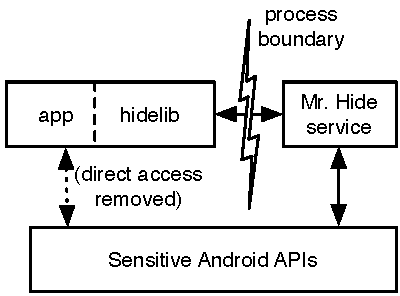
\includegraphics[width=2in]{hide-arch}
  \caption{\lib architecture}
  \label{fig:hide-arch}
\end{figure}

As discussed above, \lib provides controlled access to system
resources by interposing a new API, implemented via Android services,
between underlying resources and client apps.  
Figure~\ref{fig:hide-arch} gives an overview of the \lib architecture,
which contains two main components: the \lib service, which runs in a
separate process, and
\code{hidelib}, a drop-in replacement for sensitive Android APIs that
manages all interprocess communication with the \lib services. As
illustrated in the figure and discussed more in
Section~\ref{sec:drandroid}, \code{hidelib} is actually appended
to the original app's apk.

Before
presenting details of the \lib implementation, we first give an
overview of some aspects of the Android platform.

\subsection{Android platform overview}

Android provides a component-oriented programming model with an
associated security model~\cite{EOM09}.  An Android app consists of
four main types of components: {\em Activities} that define the user
interface screens of an application; {\em Services} that run in the
background; {\em Broadcast receivers} that await asynchronous messages
from other components, including components of other applications; and
{\em Content providers} that store data and allow access to it via a
relational database interface. Apps are typically written in Java and
compiled to Dalvik, a type and memory safe bytecode format. Each app
runs in its own Dalvik virtual machine and in its own Linux process as
a distinct user. This provides system-level isolation among Android
apps.
% Components belonging to different applications interact via remote
% procedure calls (RPC).
Apps may also include native code, although in our experience this is
uncommon (except for rendering in games).
\lib provides no special interfaces for
native code, but note that native code must still have permission to
access sensitive resources. Thus if we remove a platform permission
and replace it with a \lib permission, we can be certain the native
code no longer has the access granted by the platform permission.

\lib uses Android's permission framework to define its own set of
permissions, which apps can then request in the same way as system
permissions. These \lib permissions behave just like platform
permissions---they are displayed to the user at installation time, and
no additional permissions can be acquired at run time.  When \lib
receives a remote procedure call, it first calls a platform method,
such as
\code{checkCallingPermission()}, to check whether the caller has
the right \lib permission, and throws an exception if not.  

\paragraph*{Binding to the Mr. Hide service}
Before communicating with the \lib service via interprocess
communication, applications first must bind to the service. Moreover,
this binding process must be completed before running any code that
communicates with \lib. We found that achieving synchronous service
binding in Android is a bit tricky, because the code that binds the
service must return control to the platform before the binding becomes
available.

We experimented with several possible solutions, and found the
following approach works reliably on our devices: We perform service
binding in the app's application-level \code{onCreate()} method, which
is called as soon as the app is launched.  A service binding
established in this way exists throughout the lifetime of the app, and
will be reclaimed when the app exits.
% Also reestablished if the app is killed and restarted
In all apps we looked at, this particular \code{onCreate()} method is
either not provided (in which case we can supply our own to bind the
service), or it exists but does not contain any code that would need
to contact \lib (in which case we can chain it together with our own
method to bind the service). Then, we demote the app's ``launcher''
activity (the first to be executed when the app is started by clicking
on its icon) to a regular activity, and insert a special \lib activity
with a splash screen. The splash screen displays a message
(``Protected by \rewriter and \lib'') and then exits, passing
control onto what was the main activity. This extra interposition of
an activity causes the service binding begun in the app's
\code{onCreate()} to finish before the demoted launcher activity is
reached, thus enabling the rest of the app to assume the service is
bound.
% \jsjeon{``exits quickly, passing control'' sounds like
% it is still possible that app starts before service is ready.
% The reason \lib's launcher exits quickly is to expire service binding request.
% And then, \lib's launcher got the control back via callback from service.
% In this way, we can make sure service is indeed ready,
% starting app's original laucher activity.}

Note that there are ways to start an app without invoking its launcher
activity, e.g., intents can be used to invoke non-launcher activities
from another app. However, these are less commonly used, and \lib
could handle these cases by adding suitable logic to bind the service
if needed before these other activities execute.

%   \jeff{Does the previous handle all cases? E.g., what if the
%   app is not started via launcher? I think it's ok to only handle some
%   ways to start the app, but we should explain what we do and don't
%   handle.}
% \jsjeon{Good point; we should mention other ways, e.g.
% widget on the home screen, services that start when the phone boots, etc.}
% \kris{In theory apps could also have intent filters that start activities other 
% than the main activity, we could handle this with more investigation and 
% experimentation, but for now I think that we make the point without 
% implementing this.}

% As applications muse use remote procedure calls to access \lib, they
% must first setup a connection to the services implementing \lib.
% Because many apps use the functionality provided by \lib in
% \code{onCreate} implementations (within Activities), service
% connections must be established before UI code is executed.  The
% Android platform provides an \code{Application} class, which is
% initialized before any Activities in the application.  To bind to
% services, apps can request a service binding in the \code{onCreate}
% method of an \code{Application} class.  (Having the services bound
% in the \code{Application}'s \code{onCreate} is safe, as long as
% the code never makes calls to \lib, however applications only use
% \code{Application} objects to maintain global state and thus have
% relatively simple \code{onCreate} functions that do not make calls
% to \lib.) Because of the platform's message queue handling, the
% request to start the \lib services won't be processed until after the
% main \code{Activity}'s \code{onCreate} function returns.  To handle this,
% it is possible to insert a splash screen which simply returns quickly
% so that the service binding request can be processed.  When the
% service is connected, the application can send an intent to start the
% main activity and the app can proceed making calls to \lib without
% interruption.
% \kris{How do I differentiate between the ``main'' activity and the
%   technically main activity (the splash screen), does it matter?}
% \jsjeon{For clarity, I think we need to distinguish them somehow,
% e.g. \lib's launcher acitivity vs. app's original launcher.
% More technically, we replace ``launcher'' activity, not main activity.
% Apps can have many activity with action \code{MAIN}, but should have
% only one activity with category \code{LAUNCHER}.
% When we click app's icon, the system finds and sends an intent to
% the activity with \code{LAUNCHER} category.
% }

\paragraph*{Parameterized permissions}
Finally, Android does not directly support parameterized permissions
such as \polInternetUrlName{$d$}, but we can encode these using a
\emph{permission tree}, which is a family of permissions whose names
share a common prefix.  For example, \polInternetUrlName{\url{google.com}}
is represented in \lib as an instance of class
\perm{hidelib.\bnsp{}permission.\bnsp{}net.\bnsp{}google\_com}, which is
part of the \perm{hidelib.permission.net} tree. Note that the permissions
provided by a service such as \lib need to be defined by the 
time that the service's clients are installed.
\lib contains a GUI for adding permissions needed by new clients, as well as 
a predefined list of useful \polInternetUrlName{\(d\)} permissions.



%is installed. For research purposes, it is easy enough to predefine
%appropriate \perm{InternetURL} permissions for the fixed set of apps
%we study in this paper.
%In practice, we could either create a
%specialized copy of \lib at app rewriting time and deploy it with the
%%app (which is probably a good design, since it limits the scope of
%any unknown flaws in \lib's implementation), or we could check
%these permissions using a different mechanism (e.g., develop our own
%custom permission API).

% Android components access sensitive system resources in one of two
% ways: either via method calls through platform APIs, or via remote
% procedure calls to a service running separately on the phone.  In all
% cases, access control checks are performed by trusted reference
% monitors running outside the requesting component's address space.

% See e.g. 
% luni/src/main/native/org_apache_harmony_luni_platform_OSNetworkSystem.cpp

% Mr. Hide libraries follow the latter approach.  Our code runs in services and
% clients communicate with them via synchronous RPC calls. While an asynchronous
% process is used to establish the synchronous binding between client
% applications and services and our APIs do not map one-to-one with
% Android APIs, the Mr. Hide client library mostly abstracts away
% these details.  In the following we briefly discuss interesting
% aspects of each implemented service the corresponding parts of the
% client library.

\subsection{Permission implementations}

\paragraph*{InternetURL($x$)} 

%Android contains several packages giving apps 
%Internet access or supproting such access, including \code{java.net},
%\code{org.apache}, \code{android.webkit}, and \code{javax.net}. 

Android apps access the Internet using libraries that wrap low-level native
code interfaces.  This native code provides
access to the Linux system call interface and the
efficient cryptographic libraries
used for SSL sockets.
\code{hidelib} virtualizes these low-level components,
implementing native calls 
declared in the classes \code{InternetAddress},
\code{OSNetworkSystem}, and \code{NativeCrypto}.  Would-be native calls are 
forwarded to a \lib service.  Structures that cannot not be marshaled for RPC, such as file handles and SSL
contexts, are represented using
unique proxy values, which the \lib services maps to, e.g., Linux file
handles.
%
\lib performs access control checks before
establishing socket connections or performing DNS lookups.
%The service
%maintains a map from dynamically discovered IP addressed to corresponding
%hostnames, a

%Then to create \code{hidelib}'s adapter for \code{java.net} and
%\code{org.apache} in \code{hidelib}, we duplicated (using source-to-source
%translation)
%the original source code of those packages, modified package names
%(so the classes would be inside \code{hidelib}) and changed code to use
%\lib's \code{OSNetworkSystem} service.

Most apps do not directly access low-level code, such as
\code{OSNetworkSystem}, and instead rely on high-level, built-in
libraries for network access.  These libraries
include
\code{java.net},
\code{org.apache}, \code{android.webkit}, and 
\code{javax.net}.  
Because these
built-in libraries are dynamically linked, we cannot modify them using
\rewriter.  Instead we build work-alike libraries by recompiling the
original source to these libraries, making suitable source-level changes both
automatically (e.g., renaming classes and methods) and manually (e.g.,
modifications to use our native code wrappers). These recompiled libraries are included in \code{hidelib}.
\code{hidelib} replaces large parts of the functionality of
\code{java.\bnsp{}net},
\code{org.\bnsp{}apache}, and
\code{javax.\bnsp{}net}. Because these interfaces are large, we do not
have complete coverage of all functions, which occasionally leads to
observable differences in apps, as mentioned in
Section~\ref{sec:overview}. We also do not support
\code{android.webkit}; later versions of the platform
include hooks for controlling webkit's use of sockets, which we believe
would be a better implementation choice for \lib than recompilation.

% Because the high-level networking interfaces are large, we do not have complete
% coverage of all functions.  For the apps we consider, this primarily affects
% Barcode and Dropbox, both of which use networking components in the Java
% security framework that we do not cover.  When rewriting Barcode for
% \perm{InternetURL} permission, users lose the ablility to search a
% book's text after scanning a barcode-encoded ISBN.  We do not rewerite
% Dropbox for \perm{InternetURL} as its tightly coupled to the unimplemented
% framework components. 
%JF: Above should be in section 3.

\paragraph*{AdsPrivate and AdsGeo}

\lib's \polAdsBlindName service provides an interface allowing clients 
to request ads from the AdMob webservice.  Standard apps use an
unrestricted \perm{INTERNET} permission to connect to the AdMob
webservice, which may send private information, such as a cookie 
%the phone's unique id,
for ad targeting.  In contrast, changing apps to use \polAdsBlindName allows apps to receive
ads without being granted arbitrary network access.

%These two permissions are implemented by creating an adapter for the
%AdMob library's API. \jeff{explain more about the API.} By virtue of
%this design, a
%client may only send a 15 character alpha-numeric string, its
%\emph{advertiser id}, to a distinguished 
%webservice (hosted at \url{googleads.g.doubleclick.net}) which responds with
%an html and javascript formatted advertisement.  Dr. Hide returns this ad to
%the client.
%The implementation of permission \polAdsGeoName is similar, except
%\lib includes a location with ad requests.

\lib manages connections to the AdMob webservice in an isolated
service process. When this process requests ads on behalf of clients,
it forwards the
developer's \emph{advertiser id} (used to credit app developers for displaying
ads), but no other information, to AdMob when requesting ads. After making
a request,
\lib receives an
an HTML formatted ad, downloads a referenced image,
marshals the image as
appropriate, and returns it to the client via a remote procedure call.
\lib does not currently support newer
ads containing javascript and multiple images, but these could be supported
similarly.
%not allways Ad formats have recently changed, and 
%can contains both javascript and references to images;
%\lib

The implementation of \polAdsGeoName is similar, except
\lib includes a location with the ad requests.  This location
is obtained by the \lib service itself,
so apps may be given \polAdsGeoName without having
access to location.
Currently this location is
precise, but could be made coarse-grained to reduce the information 
provided to AdMob.

%\jeff{how does adsgeo interact with locationblock?}

%To maintatin compatibility with legacy code, the client libraries assocaited
%with the permissions provide methods, such as, that ostensibly c

Two potential covert channels remain in this architecture: an advertiser could
use two or more ids to send binary encoded strings, or could leak
information in the timing of ad requests.  We believe these low-bandwidth
channels pose relatively minor privacy risks, and
a stricter implementation of
\polAdsBlindName and \polAdsGeoName could mitigate these channels by memoizing the
advertiser ID and requesting ads on a suitable (fixed or randomized) schedule.

\paragraph*{LocationBlock and UniqueID}

Apps typically access location data via a special
\code{LocationManager} object provided by the platform. The
\code{LocationManager} allows the programmer to request asynchronous
callbacks with current location information at programmer-selected
time intervals. To implement \perm{LocationBlock}, we provide a
replacement for \code{LocationManager} in \code{hidelib} that passes on
requests for asynchronous callbacks to the \lib service. That service
polls the location at the specified intervals (using the system
\code{LocationManager}) and then does a remote procedure call back to
\code{hidelib}'s \code{LocationManager}, which then calls the callback
specified by the app. GPS location coordinates returned by \lib are
truncated to provide approximately 150m resolution.

In a few cases, apps also use
\code{LocationManager.} \code{getLastKnownLocation()} to find location
information. \code{hidelib} returns null in this case, which is
allowed in the API and should be handled by the app.

Apps can also access the current location via a
\code{TelephonyManager} object (which finds location based on cell
network information). The same object is also used to return a unique
identifier for the device. Thus, \code{hidelib} provides a
replacement \code{TelephonyManager} object. For location information
retrieved in this way, \code{hidelib} simply returns null values,
indicating the app should get the location a different way---this case
should be handled according to the API, and was in all the apps we
studied.

To support \perm{UniqueID}, our \code{TelephonyManager}'s
\code{getDeviceId()} method returns a fixed value that is not the
device's actual id. This could easily be generalized to a range of
policies, such as returning a random value each time, returning a
per-app randomized value, returning a per-app-author randomized value,
etc.

% \paragraph*{UniqueID}

% The \perm{UniqueID} permission gives an application access to various
% personal information (phone number, unique device ID, ...) that can
% uniquely identify the device.  This information is acquired by using a
% system facility, \texttt{TelephonyManager}, which is accessed via a
% call to \texttt{getSystemService}.  Although the
% \texttt{TelephonyManager} provides unique identification information,
% the class also provides a number of other purposes.  For example, this
% class also allows an app to see which type of network the device is
% currently using for communication; this does \emph{not} require a
% permission.  As previously mentioned, some apps also use
% \texttt{TelephonyManager} to determine a coarse location.  When
% rewriting either \polLocationBlockName or \perm{UniqueID}, we replace
% the entire \texttt{TelephonyManager} class with a \lib implementation,
% which checks to see if the app has appropriate \lib permissions and
% handles the permissions specific methods accordingly and leaves all
% other methods as a thin wrapper to an underlying Android
% \texttt{TelephonyManager}.

\paragraph*{SetRingtone}

Device ringtones can be set in two ways on Android, using a
\code{RingtoneManager} object or by calling
\code{Settings.System.putString()}; the former
is actually implemented on top of the latter.
%$The \code{RingtoneManager}
%in fact, the former is a helper method that calls the latter
%with the right arguments.
Thus, to implement \perm{SetRingtone}, \code{hidelib}
provides replacement \code{RingtoneManager} and
\code{Settings.System} classes, each of which contact a \lib service
to change a ringtone when requested. 
%The \code{hidelib} variant of 
%\code{Settings.System} only modifies the \code{putString()} method, 
%and then only when used for ringtones.  

The \lib service itself a thin wrapper that checks permissions and
forwards
\code{Settings.\bnsp{}System.\bnsp{}putString()}
requests.
%Currently permissions are 
%used to guard

\paragraph*{ReadVisibleContacts}

Contacts are implemented on Android as a content provider, i.e., a
database that can be queried by apps. Content providers are accessed
by asking the platform to retrieve a particular URI that contains
both the content provider and any additional parameters to pass to
it, e.g., an app can request \code{content://contacts} to get all the
contacts on the device. For portability, apps typically derive such
URIs from predefined strings, e.g., 
\code{ContactsContract.Contacts.CONTENT\bnsp\_URI} contains the URI just
mentioned.

\lib implements a new content provider that uses the same patterns as
device Contacts, but with a different name. Then \code{hidelib}
provides replacement classes for \code{ContactsContract.Contacts} and
similar that refer to \lib's content provider. The \lib service
captures the URIs sent to the content provider, inserts extra
selection constraints to the query to filter out contacts that are
invisible, and sends the modified query to the underlying Android
content provider.

% Applications access device Contacts using an Android content provider.
% This is a general mechanism through which applications publish
% information to the rest of the system using a URI based querying
% framework, and not unique to contacts.  Content providers are queried
% using a set of URI patterns which the calling application must know.
% For portability these URIs are typically kept in libraries (and in
% this case, the Android \texttt{ContactsContract} class).  \lib
% implements a new content provider using the same URI patterns as the
% underlying Android contacts content provider, and allows the same view
% of the contacts as the standard android content provider, but filters
% out contacts that are invisible to the owner.  The implementation
% captures the URIs sent to the content provider, inserts extra
% selection constraints to the query, and sends the modified query to
% the underlying Android content provider.

\section{\rewriter}
\label{sec:drandroid}

\begin{figure}[t]
  \centering 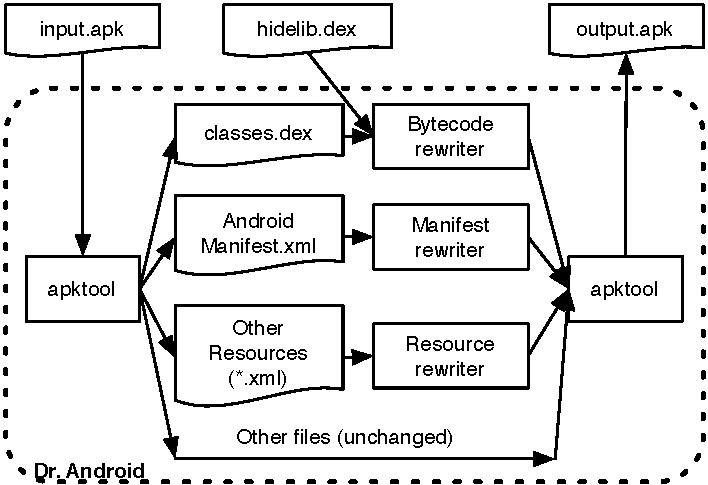
\includegraphics[width=\columnwidth]{arch}
  \caption{\rewriter architecture}
  \label{fig:arch}
\end{figure}

% \lib{} could be used as-is by security-conscious developers to reduce
% the privilege level of their apps.
As discussed earlier, we developed a tool called \rewriter
that performs binary transformation of Android apps to replace Android API
calls with calls to \lib equivalents. Figure~\ref{fig:arch} shows the
architecture of \rewriter. Given an input apk file, \rewriter
uses \code{apktool}~\cite{apktool} to decompress the input
file into its constituent files and directories. \rewriter then
performs three kinds of transformations. First, it modifies
\code{classes.dex}, the file that contains the Dalvik bytecode for
the app, to use \lib; in the process, \rewriter also concatenates \code{hidelib.dex},
an adapter layer to connect to the \lib service running in a separate
process, to the output \code{classes.dex} file. Second, \rewriter
modifies the list of permissions in \code{AndroidManifest.xml}, the
application's \emph{manifest}, which
contains the permissions requested at app installation time. In some
cases, \rewriter also must modify some additional XML files
(details below). All of the modified files, as well as the remaining
files in the app (e.g., images, data files, etc) are then repackaged
using \code{apktool} to produce a transformed apk.

Note that we need to digitally sign \code{output.apk} to run it on a
phone. It is easy to generate a key to sign apps, but it will
unavoidably differ from the key for the original app. Fortunately,
app signatures are mostly used to establish trust relationships
between different apps signed by the same key. We can
preserve these relationships by consistently signing apps from the
same original authors with the same new key.

%Permission
Manifest and resource rewriting are quite straightforward. Existing
permissions appear as \code{$<$permission$>$} elements in
the manifest, and so those elements are modified as
necessary to refer to the appropriate \lib permissions.
%
We also modify the launcher \code{$<$Activity$>$} to be an ordinary, non-launcher
activity, and insert \lib's splash screen activity.
% In order to have apps bound to \lib's services before proceeding to
% their own functionalities, class names in the \code{$<$Application$>$}
% element and \code{$<$Activity$>$} with \texttt{LAUNCHER} category
% should be replaced with \lib's equivalents.
%
Similarly, resource rewriting simply involves modifying some
elements in XML files. Resource rewriting is only used to support
\polAdsBlindName and \polAdsGeoName, and is explained in more detail in
Section~\ref{sec:specific-xform}. Thus, most of the challenge in
\rewriter is in transforming Dalvik bytecode files.

\subsection{Transforming bytecode files}

Dalvik bytecode files are structured as a series of indexed ``pools''
that contain, among others, strings, types, field signatures, method signatures,
classes, field definitions, and method definitions.\footnote{Note that
  unlike in the Java Virtual Machine, in which each class is compiled
  to separate file, in Dalvik all the classes for an app appear in the
  same \textsf{.dex} file.}  The various pools are tightly intertwined,
with many pointers from one to another, e.g., a method signature
contains a list of pointers to the type pool, and the type pool contains
pointers to elements in the string pool (containing the actual type names).
Dalvik bytecode instructions (which appear
in method definitions) often refer to elements in various pools, e.g.,
method invocation instructions include a pointer to a method
signature.
Before the Dalvik Virtual Machine executes a bytecode
file, it first \emph{verifies} it to check that, among other things, the file is
well-formed and the method bodies are type safe.

The bytecode transformer in \rewriter comprises approximately 10K
%\jsjeon{10,290 w/ ext., 8,269 w/o ext.}
lines of OCaml code that parses a bytecode file into an in-memory data
structure, modifies that data structure, and then unparses it to
produce an output bytecode file. We designed our in-memory
representation to be as faithful as possible to the on-disk
representation, to make the input and output process easy.

\begin{figure}[t]
\begin{lstlisting}[numbers=left, frame=single, xrightmargin=-2pt]
type perm = AdsPrivate | AdsGeo | ...
let (perm_map : perm -> (string * string) list) = ... /** \label{line:perm-map} */
let (perm_manager : perm -> (string * string) list) = ... /** \label{line:perm-manage} */

let rewrite (dx : dex) (ps : perm list) : unit =
  merge_hidelib dx; /** \label{line:merge} */
  replace_classes dx (List.concat (List.map perm_map ps)) /** \label{line:class_repl} */
  if (List.mem AdsPrivate ps || List.mem AdsGeo ps) then /** \label{line:elide-begin} */
    elide_perm_checks dx ["android.Permission.INTERNET"; 
      "android.Permission.ACCESS_FINE_LOCATION";
      "android.Permission.ACCESS_COARSE_LOCATION"];/** \label{line:elide-end} */
  replace_managers dx ps perm_managers; /** \label{line:manager-replace} */
  if List.mem ReadVisibleContacts ps then /** \label{line:contact-begin} */
    replace_contact_strings dx; /** \label{line:contact-end} */
  insert_service_binding dx /** \label{line:service} */
\end{lstlisting}
\caption{Bytecode rewriter pseudocode}
\label{fig:redexer-func}
\end{figure}

% AdsPrivate, AdsGeo, InternetURL(x), LocationBlock,
% PhoneStatusListener, ReadContactGroup(g), SDCardOwnFiles,
% SDCardShared, SetRingtone, UniqueID

Figure~\ref{fig:redexer-func} gives slightly simplified OCaml code for
a function \code{rewrite} that applies \lib-specific modifications
to its argument \code{dx}, the data structure (of type \code{dex})
representing a bytecode file. (Note that we chose to modify this data
structure by side effects rather than using a purely functional
implementation because it was slightly simpler.) The second argument,
\code{ps}, is the list of \lib permissions for which the app should be rewritten.

This function begins by calling \code{merge\_hidelib} to append the
contents of \code{hidelib.dex} to \code{dx}. This is not quite as easy
as it sounds, because the Dalvik verifier requires that each
of the pools in a bytecode file are both duplicate-free and
sorted. For example, there must be at most one string \code{V}
representing the type void in the type pool, but it is almost
guaranteed this type appears in both the app's code and
\code{hidelib.dex}. In our implementation, we permit a \code{dex} data
structure to contain duplicates and out-of-order elements, and we
re-sort and eliminate duplicates in each pool before producing the
output file.

Next, on line~\ref{line:class_repl} we call \code{replace\_classes} to
change references to Android platform code to refer to
\code{hidelib.dex} instead. As mentioned earlier, we designed the \lib
adapter layer to
provide drop-in replacements for platform APIs. Thus, the
input to \code{replace\_classes} is a map from platform API
class names to the corresponding \code{hidelib.dex} class names, which is then used
to modify all references to that type, e.g., in instructions, field or
method signatures, debugging information, annotations, etc..
For example, to support \polAdsBlindName
\rewriter transforms accesses to
\code{com.admob.android.ads.AdView} with accesses to a class
\code{hidelib.ads.clientsideonly.AdView}, among many others.
Here, the mappings are represented with associative
lists, and \code{perm\_map} is defined on line~\ref{line:perm-map} as a
function that, given a permission, returns its corresponding
mapping. The mappings for every permission in \code{ps} are
simply concatenated together on line~\ref{line:class_repl}.

Note that \code{replace\_classes} does not replace references inside
code from \code{hidelib.dex}. This lets us neatly handle the case when
one class has both privileged and unprivileged methods; the privileged
method wrapped in \code{hidelib.dex} contacts the \lib service, and the
unprivileged methods call into the platform as usual, and hence we do
not rewrite those calls. % (We could instead have created a
% \code{replace\_methods} function, but then we would need to statically
% analyze dynamic dispatch to know which method invocations to rewrite.)
%JF: Above paragraph could be cut

Then, on lines~\ref{line:elide-begin}--\ref{line:contact-end}, we
modify some code to support \perm{AdsPrivate}, \perm{AdsGeo},
\perm{LocationBlock}, \perm{SetRingtone}, and \perm{ReadVisibleContacts}; we defer discussion of these
modifications until we talk about those permissions in
Section~\ref{sec:specific-xform}.
Finally, on line~\ref{line:service} we insert code to bind the
\lib service (running in a separate process) so it can be called
from the app. As discussed earlier, we place this code in the
application-level \code{onCreate()} method.
More specifically, apps specify this
\code{onCreate()} method by naming its containing class in the
manifest. If such a class is defined, we modify it so
its superclass is \code{hidelib.Application},
which will ensure \lib's \code{onCreate()} is called.
Otherwise, we simply extend the manifest to name
\code{hidelib.Application} as the class containing the
application's \code{onCreate()}. Additionally, recall that after \lib's
\code{onCreate()} runs, it starts a splash screen.
The call to \code{insert\_service\_binding} stores the name of the
app's original launcher activity in a designated string, and the
splash screen code in \lib{} uses that name to reflectively launch
that activity when it exits.

% \jeff{I don't understand the following. How does the splash screen
%   activity know which other activity to launch?}
% \jsjeon{like reflection! an activity can start another activity
% only using that activity's class name and package name.
% We placed bogus strings for those, and then replace those with
% the target app's ones.}
% For easy bytecode rewriting, \lib's launcher activity uses a string-based
% intent to start app's original launcher activity.
% Such intent is composed of a package name and a class name,
% and we simply replace those with app's package name and
% launcher activity name, which are in the manifest.

% \jsjeon{need to explain either (or both?) Activity.onCreate()
% or Application.onCreate(), where \rewriter{} inserts service binding.}
% By inserting RPC bindings in all activities with reference counting,
% apps can hold a service connection of which duration is exactly same
% as apps' life cycle.  But, this approach impedes developing other
% permissions.  On the other hand, inserting an RPC binding in app's
% application instance is much simpler: it does not require reference
% counting because one and only service connection is guaranteed.
% Adding new permissions becomes simpler as well, since all service
% bindings are gathered and managed within application.onCreate().
% The only drawback of this approach is it cannot release the service
% connection.  Since app's life cycle highly depends on system's
% decision, which takes various environments into accounts, this
% approach cannot decide when to release the service binding.  However,
% it is ignoreable in that it does not affect user experience; some
% complaining messages would remain in logcat, though.  Note that, in
% some sense, we thought such leak of service binding is bad things,
% and came up with reference counting, but leaving the service
% connection as garbage seems fine in the users' viewpoint.
% \jsjeon{last sentence is not that good for paper; need to polish}

Next, we discuss in more detail the rewrites necessary for each of
\lib's new permissions.

\subsection{\lib-specific rewrites}
\label{sec:specific-xform}

\paragraph*{InternetURL}
As mentioned earlier, \code{hidelib} provides an interface that replaces
\code{java.net} and \code{org.apache}. Thus, the
transformation that replaces \perm{INTERNET} permission with various
\perm{InternetURL($d$)} permissions modifies references to those
packages to simply refer to \lib instead.

\rewriter includes a tool that finds all URL-like strings appearing in
an app's string pool. Then when we add \perm{InternetURL($d$)}
permissions to an app, we do so for all such strings. In our
experience, this allows apps to run correctly, while at the same time
greatly restricting their access to the Internet. 
%TODO: remove urls for admob

\paragraph*{AdsPrivate/AdsGeo}
As expected, the transformation for \perm{AdsPrivate} and \perm{AdsGeo}
replaces calls to the AdMob library with
appropriate \lib{} equivalents. Interestingly, there are two
additional steps needed to make ads work.

First, we discovered that AdMob checks
for the presence of the \perm{INTERNET} permission, and disables
display of ads if not present. Some apps that use these libraries also
check for \perm{ACCESS\_FINE\_LOCATION} and
\perm{ACCESS\_COARSE\_LOCATION}, to determine whether to show
localized ads.  Thus, \rewriter disables these permission checks.  In
Figure~\ref{fig:redexer-func},
lines~\ref{line:elide-begin}--\ref{line:elide-end} call a function
\code{elide\_perm\_checks} that takes a list of permission names and
replaces checks for those with no-ops. Specifically, it finds code
sequences with the following pattern, where \code{@str\_id} is the
(index of the) target permission string, and \code{@mtd\_id} refers to
the method \code{Context.checkCallingOrSelfPermission}:
\begin{lstlisting}[xleftmargin=1em]
const$\textrm{-}$string v_x @str_id
invoke$\textrm{-}$virtual this, v_x, @mtd_id
move$\textrm{-}$result v_y
\end{lstlisting}
\code{elide\_perm\_checks} replaces the last instruction in the sequence with
\begin{lstlisting}[xleftmargin=1em]
move$\textrm{-}$const v_y 0
\end{lstlisting}
where constant 0 means \code{PERMISSION\_GRANTED}.

Second, we found that apps often contain XML files that
customize the screen layout for ads under a range of different screen
resolutions. These files contain references to 
\code{com.google.ads.GoogleAdView} and other ad-related classes, and
thus we modify those to refer to \lib's ad classes.
This is equivalent to class replacement in
\code{.dex} files, except here we need to replace
classes that appear textually in XML files.

% Application resources, such as layout or strings, can be externalized
% in order to support various settings.\footnote{\url{http://developer.
% android.com/guide/topics/resources/providing-resources.html}}
% For different settings, e.g. resolution, view elements from 3rd
% party ads libraries can be defined in such external resources.
% \rewriter{} searches app's layout definitions and replaces those
% view elements with \lib{} equivalents.

One additional challenge we encountered in supporting ad permissions
is that two apps (Shazam and Advanced Task Killer)
had been obfuscated by
changing class and method names. This is not a problem with
transformations for platform APIs, since those names cannot be
changed; but ad libraries are statically linked into apps, and so
their classes and methods can be renamed. To solve this problem, we
developed a simple tool that matches up method signatures between
obfuscated and unobfuscated AdMob interfaces (the obfuscation did not
change these signatures). Using the output of this tool, we can then
direct \rewriter to transform the correct set of ad API calls to use
\lib instead. This approach allowed us to deobfuscate Shazam and Advanced Task
Killer sufficiently to support ad permissions.

\paragraph*{LocationBlock and UniqueID}

As mentioned earlier, apps access locations via either a
\code{LocationManager} or \code{TelephonyManager} object; the latter
is also used to find the device ID. Apps request
these objects by calling the platform function \code{getSystemService()},
which takes as its argument a string describing the type of
manager needed (location, telephony, etc.). The
\code{getSystemService()} method then returns
a generic Java \code{Object} that must be downcast to a
\code{LocationManager} or \code{TelephonyManager}, as appropriate.
\rewriter detects this cast and replaces it
with a call to \code{hidelib.dex} to create a manager object of the
appropriate type. Notice that this cast detection trick avoids the need for a
separate static analysis to discover which calls to
\code{getSystemService()} return which managers (or objects for other services
unrelated to location or telephony).
% (note this
%call will succeed even if the app does not have permission to access
%locations). 
Since requests for locations and unique ids all go through the
\code{LocationManager} and \code{TelephonyManager} objects, once we replace those we need not
modify any other part of the class.
%
In Figure~\ref{fig:redexer-func}, this \code{LocationManager}
substitution is performed by the calls to \code{replace\_managers} on
line~\ref{line:manager-replace}. In addition to the \code{dex} data
structure, this function takes the list of permissions and a function
\code{perm\_managers} that defines which managers need to be
substituted for each permission. For example, \code{perm\_manager
  LocationBlock} would return a list mapping Android's \code{LocationManager}
and \code{TelephonyManager} to \code{hidelib}'s equivalents.

\paragraph*{SetRingtone}

Apps change the phone's ringtone using a \code{RingtoneManager}, and
so as above, we replace such an object returned from
\code{getSystemService()} with the corresponding object from \lib. As
above, this occurs on line~\ref{line:manager-replace}.

\paragraph*{ReadVisibleContacts}
As discussed earlier, contacts are implemented as a content provider,
accessed via URIs that are usually constructed from constant strings
defined in the platform API. \code{hidelib} contains replacements for
those classes, so to change an app to use \perm{ReadVisibleContacts},
we change references to the API classes containing contact URIs to the
\code{hidelib} classes. We found that some apps also hard code the URIs
instead of using platform classes, so to support these cases \rewriter
also searchers for contact-related URI strings in the string pool and
modifies them
appropriately. Lines~\ref{line:contact-begin}--\ref{line:contact-end}
in Figure~\ref{fig:redexer-func} perform this rewriting.


% \jeff{Review this}
% Accessing Contacts is done using a general Android mechanism known as
% a content provider.  These are abstractions of a database which use a
% URI based querying interface: each content provider has a URI which it
% exposes to the entire system, possibly requiring the app accessing the
% provider to have a specific permission.  Android uses a
% \code{ContactsContract} class which specifies the different URIs and
% options used to access the Contacts content provider.  We rewrite apps
% to use a custom \code{ContactsContract}.  Some apps hard code the URIs
% of the content providers instead of using the \code{ContactsContract},
% in which case we search and replace strings in the file and modify
% them to use the strings for our replacement content provider.  Because
% the contacts API changed in an earlier implementation of Android, some
% apps still use the deprecated contacts API for compatability purposes:
% \lib doesn't implement this API, but could in theory.

% \begin{verbatim}
% RingtoneRewrite() {
%   MergeACPlib();
%   replace_classes(Android_contact_contract_classes, ACPlib_contact_contract);
% }
% \end{verbatim}

\section{Experiments}
\label{sec:eval}

We evaluated the combination of \lib and \rewriter in three ways. 
First, we performed informal testing on \lib to ensure it implements all
its permissions correctly. For example, we tested using \lib to access
contacts and verified that only visible contacts were revealed, and
similarly for the other permissions.  As these particular results are not very
interesting, we do not report on them further.
Second,
we used microbenchmarks to measure the overhead of using \lib and
\rewriter compared to using direct system calls.
%
%
Third, we ran
\rewriter on the apps discussed in Section~\ref{sec:overview} and
evaluated the correctness and usability of the transformed apps, using
a purpose-built automated testing framework in conjunction with manual
tests.



\subsection{Microbenchmark performance}
\label{sec:micro}


\begin{figure}[t!]
  \centering
  \small
  \rowcolors{1}{white}{lightgray}
  \begin{tabular}{|lrrr|} \hline
    \multicolumn{1}{|c}{\textbf{Task}} &
    \multicolumn{1}{c}{\textbf{Orig (s)}} &
    \multicolumn{1}{c}{\textbf{Transformed (s)}} &
    \multicolumn{1}{c|}{\textbf{Slowdown}} \\ \hline
    Internet & 16.241 & 20.252 & 25\% \\
    Location & 15.004 & 19.407 & 29\% \\
    Ringtone &  1.257 &  1.382 & 10\% \\
    Contacts &  0.634 &  0.953 & 50\% \\ \hline
%    SDCardWrite & ? & ? & ?\% \\ \hline
  \end{tabular}
  \caption{Microbenchmark performance results}
  \label{fig:microbenchmark}
\end{figure}


To measure the overhead of the interprocess communication entailed by
\lib, we developed a set of microbenchmarks as Android
activities that retrieve data from a sequence of 100
distinct web pages on the local network; request 10 location updates;
change ringtone paths 1,000 times; and make 100 queries to the contact
manager.   

Figure~\ref{fig:microbenchmark} shows the running times of these
microbenchmarks before and after applying \lib{} and \rewriter{}, and
the slowdown ratio.  These results are the average of 5 runs on a
Google Nexus S phone. As could be expected, the slowdowns are
fairly significant, as the interprocess communication required by \lib
is quite an expensive operation. Nevertheless, the cost of this overhead is
incurred only at relatively infrequent calls into system-level code, and
it is rarely an issue in
%issue in 
practice, as discussed below.

\subsection{\lib and \rewriter on real apps}

\begin{figure*}[t!]
\newcommand{\amazon}{Amazon}
\newcommand{\angrybirds}{Angry Birds}
\newcommand{\angrybirdsrio}{Angry Birds Rio}
\newcommand{\astro}{ASTRO}
\newcommand{\barcode}{Barcode (zxing)}
\newcommand{\bubbleblast}{Bubble Blast}
\newcommand{\bubbleblasttwo}{Bubble Blast 2}
\newcommand{\dropbox}{Dropbox}
\newcommand{\espn}{ESPN ScoreCenter}
\newcommand{\flashone}{Flashlight}
\newcommand{\flashtwo}{Brightest Flashlight}
\newcommand{\freemusic}{FreeMusic}
\newcommand{\gasbuddy}{Gas Buddy}
\newcommand{\horoscope}{Horoscope}
\newcommand{\mpring}{MP3 Ringtone}
\newcommand{\shazam}{Shazam}
\newcommand{\stardroid}{Google Sky Map}
\newcommand{\taskkiller}{Advanced Task Killer}
\newcommand{\words}{Words With Friends}
\newcommand{\amazonAut}{--}
\newcommand{\amazonMan}{15}
\newcommand{\angrybirdsAut}{--}
\newcommand{\angrybirdsMan}{2}
\newcommand{\angrybirdsrioAut}{--}
\newcommand{\angrybirdsrioMan}{2}
\newcommand{\astroAut}{13}
\newcommand{\astroMan}{17}
\newcommand{\barcodeAut}{7}
\newcommand{\barcodeMan}{8}
\newcommand{\bubbleblastAut}{6}
\newcommand{\bubbleblastMan}{8}
\newcommand{\bubbleblasttwoAut}{5}
\newcommand{\bubbleblasttwoMan}{12}
\newcommand{\dropboxAut}{8}
\newcommand{\dropboxMan}{6}
\newcommand{\espnAut}{--}
\newcommand{\espnMan}{4}
\newcommand{\flashoneAut}{--}
\newcommand{\flashoneMan}{1} 
\newcommand{\flashtwoAut}{--}
\newcommand{\flashtwoMan}{1} 
\newcommand{\freemusicAut}{--}
\newcommand{\freemusicMan}{6}
\newcommand{\gasbuddyAut}{15}
\newcommand{\gasbuddyMan}{13}
\newcommand{\horoscopeAut}{--}
\newcommand{\horoscopeMan}{11}
\newcommand{\mpringAut}{--}
\newcommand{\mpringMan}{7}
\newcommand{\shazamAut}{10}
\newcommand{\shazamMan}{10}
\newcommand{\stardroidAut}{4}
\newcommand{\stardroidMan}{5}
\newcommand{\taskkillerAut}{3}
\newcommand{\taskkillerMan}{3}
\newcommand{\wordsAut}{--}
\newcommand{\wordsMan}{13} 
  \centering
  \small
  \rowcolors{1}{white}{lightgray}
  \begin{tabular}{|l|rrr|rr|rrr|} \hline
    \multicolumn{1}{|c|}{\textbf{Name}} &
    \multicolumn{1}{c}{\textbf{Apk (KB)}} &
    \multicolumn{1}{c}{\textbf{Dex (KB)}} &
    \multicolumn{1}{c|}{\textbf{\# Ins}} &
    \multicolumn{1}{c}{\textbf{\# Chg}} &
    \multicolumn{1}{c|}{\textbf{Tm (s)}} &
    \multicolumn{1}{c}{\textbf{\# Acts}} &
    \multicolumn{1}{c}{\textbf{\# Aut}} &
    \multicolumn{1}{c|}{\textbf{\# Man}}
    \\ \hline
\taskkiller & 98 & 110 & 6,724 & 115 & 7.51 & 3 & \taskkillerAut &
\taskkillerMan \\
\amazon & 2,288 & 1,607 & 114,673 & 178 & 36.24 & 28 & \amazonAut &
\amazonMan\\
\angrybirds & 17,111 & 254 & 24,212 & 354 & 22.75 & 2 & \angrybirdsAut &
\angrybirdsMan \\
\angrybirdsrio & 12,835 & 203 & 18,539 & 274 & 21.56 & 2 & \angrybirdsrioAut &
\angrybirdsrioMan \\
\astro & 2,241 & 1,176 & 112,342 & 135 & 20.01 & 29 & \astroAut & \astroMan \\
\barcode & 496 & 454 & 64,045 & 315 & 15.65 & 9 & \barcodeAut & \barcodeMan \\
\bubbleblast & 1,413 & 714 & 66,189 & 1,013 & 17.27 & 11 & \bubbleblastAut &
\bubbleblastMan \\
\bubbleblasttwo & 4,489 & 879 & 82,233 & 1,063 & 24.34 & 16 &
\bubbleblasttwoAut & \bubbleblasttwoMan \\
\flashtwo & 1,752 & 1,857 & 173,172 & 1,289 & 27.85 & 6 & \flashtwoAut &
\flashtwoMan \\
\dropbox & 1,137 & 1,040 & 94,367 & 4,111 & 13.35 & 12 & \dropboxAut &
\dropboxMan \\
\espn & 1,483 & 670 & 57,541 & 608 & 26.48 & 5 & \espnAut & \espnMan \\
\flashone & 1,665 & 464 & 44,592 & 581 & 18.80 & 6 & \flashoneAut &
\flashoneMan \\
\freemusic & 539 & 655 & 59,111 & 676 & 10.70 & 12 & \freemusicAut &
\freemusicMan \\
\gasbuddy & 1,359 & 853 & 74,240 & 709 & 23.59 & 22 & \gasbuddyAut &
\gasbuddyMan \\
\stardroid & 2,125 & 415 & 29,401 & 81 & 17.32 & 6 & \stardroidAut &
\stardroidMan\\
\horoscope & 3,023 & 815 & 88,760 & 698 & 29.33 & 26 & \horoscopeAut &
\horoscopeMan \\
\mpring & 428 & 373 & 44,014 & 50 & 10.20 & 11 & \mpringAut & \mpringMan \\
\shazam & 1,130 & 756 & 89,310 & 661 & 21.60 & 19 & \shazamAut & \shazamMan \\
\words & 5,314 & 2,718 & 223,620 & 1,226 & 61.18 & 38 & \wordsAut & \wordsMan
\\

  \hline
  \end{tabular}
  \caption{\lib and \rewriter results on apps}
  \label{fig:exp}
\end{figure*}

Using a combination of automated and manual testing, we evaluated
if and how rewriting changes the behavior of the apps discussed in Section~\ref{sec:overview}.  We used \rewriter's
reporting features and the \troyd framework (described below) to track test
coverage, comparing the set of activities exercised by testing with the set
declared in each application's binary. 
Figure~\ref{fig:exp} summarizes this coverage information
and gives pertinent data about the rewriting process 
for each app.


\paragraph*{Scope and correctness of rewriting}

Our experiments show \rewriter is capable of processing commercially published
apps with acceptable performance, yielding correct Dalvik binaries.

Columns 2--4 in Figure~\ref{fig:exp} describe the size of apps before rewriting,
including the apk size, the size of
\code{classes.dex} after the apk is unpacked, and the number of
Dalvik bytecode instructions. % (Note that in a few
% cases, the decompressed Dalvik is actually larger than the
% apk.)
The next two columns report the number of changes applied by
\rewriter and the running time of \rewriter. A single change comprises
either an instruction modification to refer to a different class; an
elision of a permission check (counts as one change); replacement of a
\code{Location}, \code{Telephony}, or \code{RingtoneManager} (again,
one change); or changing a string in the string table for another
reason (changing a content URI, or modifying the string that contains
the activity to launch after the splash screen).  Reported performance
is based on one run on a 2.5 GHz Intel Core 2 Duo with 4 GB RAM, running
Mac OS X 10.6.8.
%No app takes more than 19 seconds to transform, which is more
%than acceptable for an offline program transformation.
As the running times show, applying \rewriter is
reasonably fast, and as it is done only once, should not be a concern.

The Android platform performs lightweight bytecode verification when apps are
installed on a phone, and more thorough verification during application
runtime.  These verification phases test various well-formedness constraints on Dalvik files.
All tested apps install and run without verification errors, giving
confidence that \rewriter's transformations are structurally correct.

\paragraph*{Automated and manual testing methodology}

%#\paragraph*{Automated regression testing}


%We by developing regression tests with 
To evaluate the behavior of rewritten apps,
we developed an automated testing framework, \troyd, 
%a new
%automated Android testing framework that we developed 
concurrently
with this work. We describe \troyd only briefly, as it is not the
focus of this paper. The key novelty of \troyd is that it can run on
apps without source code, yet it allows test writers to refer to GUI
elements by name
or text content. Test cases---written as Ruby
scripts---control apps by
injecting key events like back or menu button clicks, and can click or
edit attributes of all \code{View} elements on the screen at run
time. Test cases can also get attributes of \code{View} elements (e.g.,
contents of text boxes), which can be used to write assertions.
\troyd currently does not support clicking absolute screen locations
or dragging, which limits its applicability to some apps such as
games; we perform additional manual testing in these cases.

% Android supports testing automation by \code{monkey}, a key event
% generator, and \code{Instrumentation} package.  Key event generation
% would be useful when simulating users interactions, but it has two
% critical drawbacks: it depends on absolute coordinates and timing,
% which may vary from device to device.  On the other hand,
% \code{Instrumentation} allows us to control apps via relatively
% high-level commands and capture the snapshot of run-time instances
% because it is literally instrumented into the tested apps.
% Android has a set of instrumentation-related classes that
% support unit testing, but the way they are used requires source codes,
% which conflicts with our case.  In this regard, our testing framework
% has its own novelty in that it is able to control apps without sources
% and implemented only using Android ingredients, such as
% \code{IntentService}, \code{BroadcastReceiver}, and \code{Instrumentation}.

% \troyd{} is composed of an app that acts as a controller in the device
% and scripts that support high-level commands for easy testing,
% record testing scenarios, and interact with Android tools,
% e.g. \code{adb}, \code{aapt}, etc.  That app has an \code{IntentService}
% that receives the target app's package name as intent and
% launches that target app, a \code{BroadcastReceiver} that receives
% commands as intent, and an \code{Instrumentation} that indeed
% manipulates the target app according to the commands.
% After experiencing some designs, we settled on this because of
% such components' restrictions: only \code{Service} and \code{Activity}
% can start \code{Instrumentation}, but sending an intent to them
% via \code{am} command of \code{adb} creates a new process, which
% prevents us from controlling the target app.
% Currently, \troyd{} commands can gain \code{Activity} instances
% opened so far, inject key events like back or menu buttons, and click,
% get, or edit attributes of all \code{View} elements on the screen
% at run-time.

% To run the target app on the \code{Instrumentation}, such controlling
% app should specify the package name of the target app, and both apps,
% one for instrumentation and the other for testing, should be signed
% with the same key chain.  Along with such controller, \troyd{} has
% a rich set of scripts that automate above process, record commands,
% generate a test script for regression tests, and automatically run
% such test scripts with rewritten apks.

%\paragraph*{Test setup}

We wrote test cases for our apps with the goal of covering as many
of an app's \code{Activity}s as possible.  Each Android \code{Activity}
displays its own user interface screen to the user and so represents
a distinct piece of functionality supported by the app.  We manually
experimented with each app to understand the behavior of 
each of its activities.  We then developed tests in \troyd to 
verify that the expected buttons, menus, and other displays (e.g.,
ads) appear on an activity's UI and that clicking on these items produces
the expected behavior (e.g., displaying a different \code{Activity},
quitting the application, etc.). We ran our automated tests on a Google
Nexus S phone.

%\paragraph*{Test results}

Some activities are not
covered by \troyd for various reasons, including 
dead code (i.e., unreachable activities), activities that are not easy to
automatically test (e.g., sign up screens that would require creating fake
logins to repeatedly test), activities that require clicking absolute screen
locations or dragging, activities that are launched in a separate process
(and hence cannot be controlled by \troyd), and activities that are
tedious to reach with automated tests.



% \jsjeon{Instrumentation work only in the same process;
% by sending an intent to the photo gallery,
% that photo gallery will start as a separate process,
% so I said, \troyd lose the control---can't send any commands}

% Since we do not have source codes for apps, conventional metrics,
% such as line or branch coverage, do not work for our case.
% Instead, we come up with a new metric, called activity coverage;
% we tried to cover as many activities in apps as possible when
% designing test cases.  It is feasible for us to measure this metric
% because, thanks to \code{Instrumentation}, we can know exactly
% what activities are opened so far.  The reason we chose \code{Activity}
% as metric is, unlike other components, that is used to interact
% with users most frequently.  Hence, the more activities we cover,
% the more likely it is that our test cases reflect app's behavior
% enough in the viewpoint of users.

% The last two columns in figure~\ref{fig:exp} show the number of all
% activities each app has and the number of activities that covered by
% automatic testings.  Note that the number of all activities include
% even dead codes, and that the number of covered activities does not
% count non-repeatable tests, like sign-up process.  That is, covered
% activities only reflect reproducible automatic tests.
% Question marks mean those apps cannot be testd by \troyd{},
% and the remaining activities are handled by hand as well.

% Although we believe our testing framework is powerful enough to
% automate regression tests for \lib{} and \rewriter{}, we tested
% some apps manually, due to the limitations of \troyd{}.
% %
% It cannot click on arbitrary positions on the screen, so we cannot
% test apps that have their own views, which might hide elements inside
% them.  Most of games heavily relies on a single view for board along
% with native codes, so once such view is loaded, we cannot proceed further.
% However, we can reach, at least, to such own views by automated scripts,
% e.g. for Bubble Blast, we can check Ads are on the screen before reaching
% the game board.  Technically, we can do so as \code{monkey} event generator
% does, and leave it as a future work.
% %
% In a similar sense, \troyd{} cannot generate a sequence of events
% that mimics dragging.  That's why we cannot play Angry Birds automatically,
% but, unfortunately, there are some apps that need dragging to enable
% some features.  For example, ASTRO has an ability to access to arbitrary
% servers via sftp ports, but there is no way to reach that feature,
% except for dragging the top menu with several images.
% %
% Once apps yield the control by sending intents to other services,
% \troyd{} loses the control of the target apps, and cannot control
% that recipients.  Many apps often send intents to the browser to
% access to external resources, or to the gallery or file manager to
% browse photos or files.  For instance, Dropbox, Facebook, and Gas
% Buddy browse photos before uploading them, and \troyd{} cannot
% go further because testing would become out of control.

% Besides, there are more cases that we cannot handle via automatic
% testings.  Some apps include dead codes, e.g. Horoscope has
% some activities for chattings, but those are part of their other apps.
% %
% Several apps have some activities for signing up.  Of course, we can
% also do as we automatically sign in to some services, but it makes
% more sense to test such functionality once by hand, rather than
% many times automatically.
% %
% Messenger apps, Kakao talk and WhatsApp, require SMS service
% to register, and that is far beyound \troyd{}'s scope.

Additionally, we 
manually tested all rewritten apps, checking for obvious changes in
performance or functionality.  For each app we attempted to visit all
accessible activities and use most features.  Again, features with
costly or annoying side effects, such as finalizing purchases using the Amazon
app or posting games scores to Facebook using the Words with Friends app, were
not tested.  
We used \troyd to log visited activities during manual testing.

The last three
columns in Figure~\ref{fig:exp} report the coverage of our test suite
in terms of activities, including the total number of
activities defined in each app and the number covered
with automated and with manual testing.  Conservatively, our automatic and
manual testing together cover at least 56\% of the activities across all apps.


\paragraph*{Behavior of rewritten apps}

During testing, we found that almost all activities of applications
function normally, with no observable changes. In more detail, all automated
\troyd tests pass---running our test suites before and after applying
\rewriter produced identical sets of passing assertions---and when we
tested the apps manually, we could detect no differences in most
activities' behavior.

As already mentioned in Figure~\ref{fig:survey-table}, we did find
some differences in certain activities that use the Internet, due
to limitations of \lib.  First, ESPN ScoreCenter, Google Sky Map, and
Shazam use a WebView widget, which we do not support; these views show
placeholder text after rewriting.  % \jeff{what is the consequence?}
% \jsjeon{similar to web 404 pages}
Second, recall that \lib's implementation of ads renders a single
image.  We observed that this design choice causes ads containing
Javascript or multiple images to display improperly.
Finally, Barcode uses parts of the Java SSL
framework we do not cover; even so, the Barcode app still
works with \lib's \perm{InternetURL} permission, but
users lose the ability to search a
book's text after scanning a barcode-encoded ISBN.  In general,
  we think these differences may be acceptable to users in exchange for the increased
  security provided, and we expect that further engineering would
  eliminate them.

% Often user experience degrades gracefully, with particular parts of an
% app inaccessible, but with unrelated functionality intact.  For
% instance ESPN ScoresCenter, Google Skymap, and Shazam use a WebView
% widget to display some html-formatted information, but these views
% show placeholder text after rewriting.  In several apps, \lib renders
% some ad contents incorrectly.  While \lib supports SSL encrypted
% sockets, Barcode and Dropbox use parts of the Java security framework
% we do not cover.  We continue to transform Barcode for
% \perm{InternetURL} permission, but users lose the ablility to search a
% book's text after scanning a barcode encoded ISBN.  We leave Dropbox
% with full internet access, rewriting only for \perm{UniqueID}. Finally
% Barcode uses a deprecated API for access to contacts, and we do not
% transform this API.


% Importantly, testing helps validate our security model.  
% Whenever an app called an unsupported interface it received a
% runtime exception from \lib{}, was killed by the virtual machine (for
% unsupported native methods), or---occasionally---crashed the \lib client
% library; in no case did we see an app succeed in accessing a protected
% resource by by avoiding \lib.  While this behavior 
% is expected, because we use Android's sandbox as a fallback,
% it is nevertheless reassuring to observe it in practice.
% \jeff{It sounds bad that apps crashed the library!}


Transformed apps may experience a noticeable delay on startup while
the app connects to \lib services.  After the initial connection is
established, application performance, measured by informal observation, is
similar for transformed and untransformed applications.  We speculate that this
is because the cost of using \lib is amortized over the cost of
other operations, and because the test apps are designed to be interactive,
spending a large share of time waiting for user input.


\section{Related Work}

Several other researchers have proposed mechanisms to refine or reduce
permissions in Android. MockDroid allows users to replace an
app's view of certain private data with fake
information~\cite{mockdroid}. Apex is similar, and also lets 
the user enforce simple constraints such as the
number of times per day a resource may be accessed~\cite{apex}. TISSA
gives users detailed control over an app's access to selected private data
(phone identity, location, contacts, and the call log), letting the
user decide whether the app can see the true data, empty data,
anonymized data, or mock data~\cite{zhou2011taming}. AppFence
similarly lets users provide mock data to apps requesting private
information, and can also ensure private data that is released to apps
does not leave the device~\cite{Hornyack:2011:TAD:2046707.2046780}.  A
limitation of all of these approaches is that they require
modifications to the Android platform, and hence to be used in
practice must either be
adopted by Google or device providers, or must be run on rooted
phones. In contrast, \rewriter and \lib run on stock, unmodified
Android systems available today.

Researchers have also developed other ways to enhance Android's
overall security framework. Kirin employs a set of user-defined
security rules to flag potential malware at install
time~\cite{enck2009lightweight}. Saint enriches permissions on Android
to support a variety of installation constraints, e.g., a permission
can include a whitelist of apps that may request
it~\cite{ongtang2009semantically}. These approaches are complementary
to our system, as they take the platform permissions as is and do not
refine them.

There have been several studies of Android's permissions, sensitive
APIs, and the use of permissions across apps.  Barrera et
al.~\cite{barrera2010methodology} analyze the way permissions are used
in Android apps, and observe that only a small number of Android
permissions are widely used but that some of these, in particular
Internet permissions, are overly broad (as we have also found). Vidas
et al.~\cite{vidas:w2sp11} describe a tool that, using
documentation-derived information, can statically analyze an app's
source code to find a minimum set of permissions it
needs. Stowaway~\cite{felt:ccs11} performs a static analysis on the
Android API itself to discover which APIs require what permissions,
something they found is not always well documented. (We used
Stowaway's data set in several cases to help determine what adapters
we needed to implement in \lib.)

Finally, several tools have been developed that look for security
issues in Android apps. TaintDroid tracks the flow of sensitive
information~\cite{taintdroid}. Ded~\cite{ded}, a Dalvik-to-Java
decompiler, has been used to discover previously undisclosed device
identifier leaks. ComDroid~\cite{chin11:mobisys} finds vulnerabilities
related to Intent handling. Felt et al.~\cite{felt2011permission}
study the problem of permission redelegation, in which an app is
tricked into providing sensitive capabilities to another app.
Woodpecker~\cite{grace:ndss12} uses dataflow analysis to find
capability leaks on Android phones. All of these tools focus on
improper use of the current set of Android's permissions. \rewriter
and \lib take a complimentary approach, replacing existing permissions
with finer-grained ones to reduce or eliminate consequences of
security issues.

% While our approach cannot guarantee the absence of the security
% vulnerabilities found by such tools, we believe it can help make apps
% more secure in practice.  We believe \lib{} is complimentary to such
% tools as they address different sorts of security properties.
% Furthermore, trusted libraries like \lib{} are prime candidates for
% automated validation, as reuse allows verification costs to be
% amortized and high security requirements can justify remaining per-app
% costs.

% ComDroid~\cite{chin11:mobisys} analyzes inter-application
% communication for potential security risks.  This tool could
% complement our proposed approach, which relies heavily on
% inter-application communication with trusted third parties.

% \emph{Kirin} employs a set of user-defined security rules to flag
% potential malware at install time~\cite{enck2009lightweight}.  These
% tools allow users to trade off app functionality for privacy, but they
% inherit the resource-centric nature of Android permissions, which can
% limit their effectiveness.  For example, denying Internet access to
% Google Translate would render it useless, so a MockDroid user must
% allow such access, whereas our application-centric policy provides a
% much stronger guarantee.  Moreover, our approach can be implemented
% purely as a library, with no modifications to the underlying Android
% OS. \jsjeon{cite AppFence and Stowaway?}

% {\em Saint} enriches permissions on Android to support a variety of
% installation constraints, e.g., a permission can include a whitelist
% of apps that may request it~\cite{ongtang2009semantically}.  In our
% limited experience, we have not yet needed this capability.

\section{Conclusions and Future Work}

We presented \lib and \rewriter, a pair of tools that provide
finer-grained permissions on Android without requiring any platform
modifications. \lib runs as a service, providing access to sensitive
capabilities along with a set of fine-grained permissions that grant access
to the service. \rewriter transforms apps to use \lib, operating
directly on apks to change coarse-grain platform permissions into
finer-grain \lib permissions, and modifying Dalvik bytecode to access
sensitive resources via \lib's adapter layer. We applied \lib and
\rewriter to a range of apps, and found that they leave app behavior
largely unchanged, while maintaining acceptable performance. Our
results suggest that \rewriter and \lib provide stronger privacy and
security guarantees while retaining application functionality and
performance.


\section*{Acknowledgements}

This research was supported in part by NSF CNS-1064997 and by a
research award from Google. Thanks to Philip Phelps for helping
develop the microbenchmarking app.

\bibliographystyle{abbrv}
\bibliography{refs}

\end{document}
